\documentclass[10pt,a4paper,UTF8]{ctexart}

\linespread{1.5}
\usepackage{geometry}%用于设置上下左右页边距
	\geometry{left=2.5cm,right=2.5cm,top=3.2cm,bottom=2.7cm}
\usepackage{xeCJK,amsmath,paralist,enumerate,booktabs,multirow,graphicx,subfig,setspace,listings,lastpage,hyperref}
\usepackage{amsthm, amssymb, bm, color, framed, graphicx, hyperref, mathrsfs}
\usepackage{mathrsfs}  
	\setlength{\parindent}{2em}
	\lstset{language=Matlab}%
\usepackage{fancyhdr}
\usepackage{graphicx}
\usepackage{subfloat}
\usepackage{listings}
\usepackage{xcolor}
\usepackage{float}
\usepackage{paralist}
\usepackage{setspace}
\usepackage{titlesec}
\usepackage{enumitem}
\usepackage{hyperref}
\usepackage{multirow}
\usepackage{threeparttable}
\usepackage{tcolorbox}
\usepackage{tabularx}
\usepackage{ulem}
\usepackage{multicol}
\usepackage{multirow}
\usepackage{pifont}


\hypersetup{
	colorlinks=true,
	linkcolor=black
}

\setenumerate{partopsep=0pt,topsep=0pt}
\setitemize{itemsep=0pt,partopsep=0pt,topsep=0pt}

\titlespacing*{\section}{0pt}{3pt}{3pt}
\titlespacing*{\subsection}{0pt}{2pt}{2pt}
\titlespacing*{\subsubsection}{0pt}{1pt}{1pt}
\titlespacing*{\paragraph}{0pt}{0pt}{0pt}

\setenumerate{partopsep=-2pt,topsep=-2pt,itemsep=-1pt,leftmargin=2em}
\setitemize{itemsep=-2pt,partopsep=-2pt,topsep=-1pt,leftmargin=2em}

\ctexset{secnumdepth=4,tocdepth=4}
\setlength{\parindent}{2pt}
\setstretch{1.2}


\setCJKmainfont[BoldFont={FZHei-B01},ItalicFont={FZKai-Z03}]{FZShuSong-Z01} 
\setCJKsansfont[BoldFont={FZHei-B01}]{FZKai-Z03} 
\setCJKmonofont[BoldFont={FZHei-B01}]{FZFangSong-Z02}
\setCJKfamilyfont{zhsong}{FZShuSong-Z01} 
\setCJKfamilyfont{zhhei}{FZHei-B01} 
\setCJKfamilyfont{zhkai}[BoldFont={FZHei-B01}]{FZKai-Z03} 
\setCJKfamilyfont{zhfs}[BoldFont={FZHei-B01}]{FZFangSong-Z02} 
\renewcommand*{\songti}{\CJKfamily{zhsong}} 
\renewcommand*{\heiti}{\CJKfamily{zhhei}} 
\renewcommand*{\kaishu}{\CJKfamily{zhkai}} 
\renewcommand*{\fangsong}{\CJKfamily{zhfs}}

\newcommand{\myline}{\underline{\hbox to 10mm{}}}

\definecolor{mKeyword}{RGB}{0,0,255}          % bule
\definecolor{mString}{RGB}{160,32,240}        % purple
\definecolor{mComment}{RGB}{34,139,34}        % green
\definecolor{mNumber}{RGB}{128,128,128} 

\lstdefinestyle {njulisting} {
	basewidth = 0.5 em,
	lineskip = 3 pt,
	basicstyle = \small\ttfamily,
	% keywordstyle = \bfseries,
	commentstyle = \itshape\color{gray}, 
	basicstyle=\small\ttfamily,
	keywordstyle={\color{mKeyword}},     % sets color for keywords
	stringstyle={\color{mString}},       % sets color for strings
	commentstyle={\color{mComment}},     % sets color for comments
	numberstyle=\tiny\color{mNumber},
	numbers = left,
	captionpos = t,
	breaklines = true,
	xleftmargin = 2 em,
	xrightmargin = 2 em,
	frame=tlrb,
	tabsize=4
}

\lstset{
style = njulisting, % 调用上述样式 
flexiblecolumns % 允许调整字符宽度
}


%================= 基本格式预置 ===========================
\usepackage{fancyhdr}
\pagestyle{fancy}
\lhead{操作系统}
\rhead{课后应用题作业2}
\cfoot{\thepage}
\renewcommand{\headrulewidth}{0.4pt}
\renewcommand{\theenumi}{(\arabic{enumi})}
\CTEXsetup[format={\bfseries\zihao{-3}}]{section}
\CTEXsetup[format={\bfseries\zihao{4}}]{subsection}
\CTEXsetup[format={\bfseries\zihao{-4}}]{subsubsection}


\renewcommand{\contentsname}{目录}  

\newcounter{problemname}
%以下为有题目阴影
\definecolor{shadecolor}{RGB}{241, 241, 255}
\newenvironment{problem}{\stepcounter{problemname}\vspace{-0.5em}\begin{shaded}\par\noindent\textbf{\arabic{problemname}. }}{\end{shaded} \vspace{-1em} \par}
%以下为无题目阴影
% \newenvironment{problem}{\stepcounter{problemname}\par\noindent\textbf{\arabic{problemname}. }}{\par}
\newenvironment{solution}{\noindent\textbf{解答:}\\ \indent}{\par}

\begin{document}

\setlength{\parskip}{0.65em}

\begin{center}
\LARGE\textbf{操作系统2022课后应用题作业2}
\end{center}

\begin{problem}
	假定磁盘有200个柱面,编号$0 \sim 199$,当前移动臂位于143号柱面上,并刚刚完成125号柱面的服务请求。如果请求队列的先后顺序是:86,147,91,177,94,150,102,175,130;试问:为了完成上述请求,下列算法移动臂所移动的总量分别是多少?并给出移动臂移动的顺序。
	\begin{enumerate}[label=(\arabic*)]
		\item 先来先服务算法;
		\item 最短查找时间优先算法;
		\item 双向扫描算法;
		\item 电梯调度算法。
	\end{enumerate}
\end{problem}

\begin{solution}
	\vspace{-1.5em}
	\begin{enumerate}[label=(\arabic*)]
		\item {\kaishu 先来先服务算法:}\\
			移动臂移动的总量为:$(143-86)+(147-86)+(147-91)+(177-91)+(177-94)+(150-94)+(150-102)+(175-102)+(175-102)+(175-130)=57+61+56+86+83+56+48+73+45=565$\\
			移动臂移动的顺序为:$143-86-147-91-177-94-150-102-175-130$
		\item {\kaishu 最短查找时间优先算法:}\\
		移动臂移动的总量为:$(150-143)+(150-86)+(177-86)=162$\\
		移动臂移动的顺序为:$143-147-150-130-102-94-91-86-175-177$
		\item {\kaishu 双向扫描算法:}\\
		移动臂移动的总量为:$(199-143)+(199-86)=169$\\
		移动臂移动的顺序为:$143-147-150-175-177-199-130-102-94-91-86$
		\item {\kaishu 电梯调度算法:}\\
		移动臂移动的总量为:$(177-143)+(177-86)=125$\\
		移动臂移动的顺序为:$143-147-150-175-177-130-102-94-91-86$
	\end{enumerate}
\end{solution}


\begin{problem}
	有一个磁盘组共有10个盘面,每个盘面有100个磁道,每个磁道有16个扇区。若以扇区为分配单位,现问:
	\begin{enumerate}[label=(\arabic*)]
		\item 用位示图管理磁盘空间,则位示图占用多少空间?
		\item 若空白文件目录的每个目录项占5个字节,则什么时候空白文件目录大于位示图?
	\end{enumerate}
\end{problem}

\begin{solution}
	\vspace{-1.5em}
	\begin{enumerate}[label=(\arabic*)]
		\item 该磁盘共有扇区数为$10\times 100\times 16=16000$个,所以位示图占用空间为$16000\div 8=2000$字节
		\item 当空白文件目录数大于400时,空白文件目录大于位示图
	\end{enumerate}
\end{solution}


\begin{problem}
	假设在Unix文件系统中,inode节点中分别含有10个直接地址的索引和一、二、三级间接索引。若设每个盘块有512B大小,每个盘块中可存放128个盘块地址,则
	\begin{enumerate}[label=(\arabic*)]
		\item 一个1MB的文件占用多少间接盘块?
		\item 一个25MB的文件占用多少间接盘块?
	\end{enumerate}
\end{problem}

\begin{solution}
	\vspace{-1.5em}
	\begin{enumerate}[label=(\arabic*)]
		\item 	直接盘块容量:$512\mathrm{B}\times 10 \div 1024=5\mathrm{KB}$\\
		一级间接盘块容量:$128\times 512\mathrm{B} \div 1024=64\mathrm{KB}$\\
		二级间接盘块容量:$128\times 64\mathrm{KB}=8192\mathrm{KB}$\\
		三级间接盘块容量:$8192\mathrm{KB}\times 1024=1048576\mathrm{KB}$

		1MB的文件占用10个直接盘块和128个一级间接盘块,二级间接盘块占用数量为$(1024-5-64)\mathrm{KB}\div 512\mathrm{B}=1910$个
		\item 25MB的文件占用10个直接盘块、128个一级间接盘块和$128\times 128=16384$个二级间接盘块,三级间接盘块的占用数量为$(25\times 1024-5-64-8192)\mathrm{KB}\div 512\mathrm{B}=34678$块
	\end{enumerate}


\end{solution}


\begin{problem}
	设有$n$个进程共享一个互斥段,如果:(1)每次只允许一个进程进入互斥段;(2)每次最多允许$m$个$(m\leq n)$进程同时进入互斥段。
	
	试问:以上两种情况下所采用的信号量初值是否相同?试给出信号量值的变化范围。
\end{problem}

\begin{solution}
	所采用的信号量的初值不同。

	对于(1)的情况,信号量的初始值为1,变化范围为 $[-n+1, 1]$。当没有进程进入互斥段时,信号量为1;最多可能存在$n-1$个进程等待进入互斥段,此时信号量的值为$-n+1$。

	对于(2)的情况,信号量的初始值为m,变化范围为 $[-n+m, m]$。当没有进程进入互斥段时,信号量为$m$;最多可能存在$n-m$个进程等待进入互斥段,此时信号量的值为$-n+m$。

\end{solution}


\begin{problem}
	有两个优先级相同的进程$P_1$和$P_2$,其各自程序如下,信号量$S_1$和$S_2$的初值均0。试问$P_1$、$P_2$并发执行后,$x$、$y$、$z$的值各为多少?
	\begin{lstlisting}
P1(){											P2(){
	y = 1;											x = 1;
	y = y + 3;										x = x + 5;
	V(S1);											P(S1);
	z = y + 1;										x = x + y;
	P(S2);											V(S2);
	y = z + y;										z = z + x;
}												}
	\end{lstlisting}
\end{problem}

\begin{solution}
	为了方便描述,对上述进程语句进行编号
	\begin{figure}[H]
		\centering
		\vspace{-0.5em}
		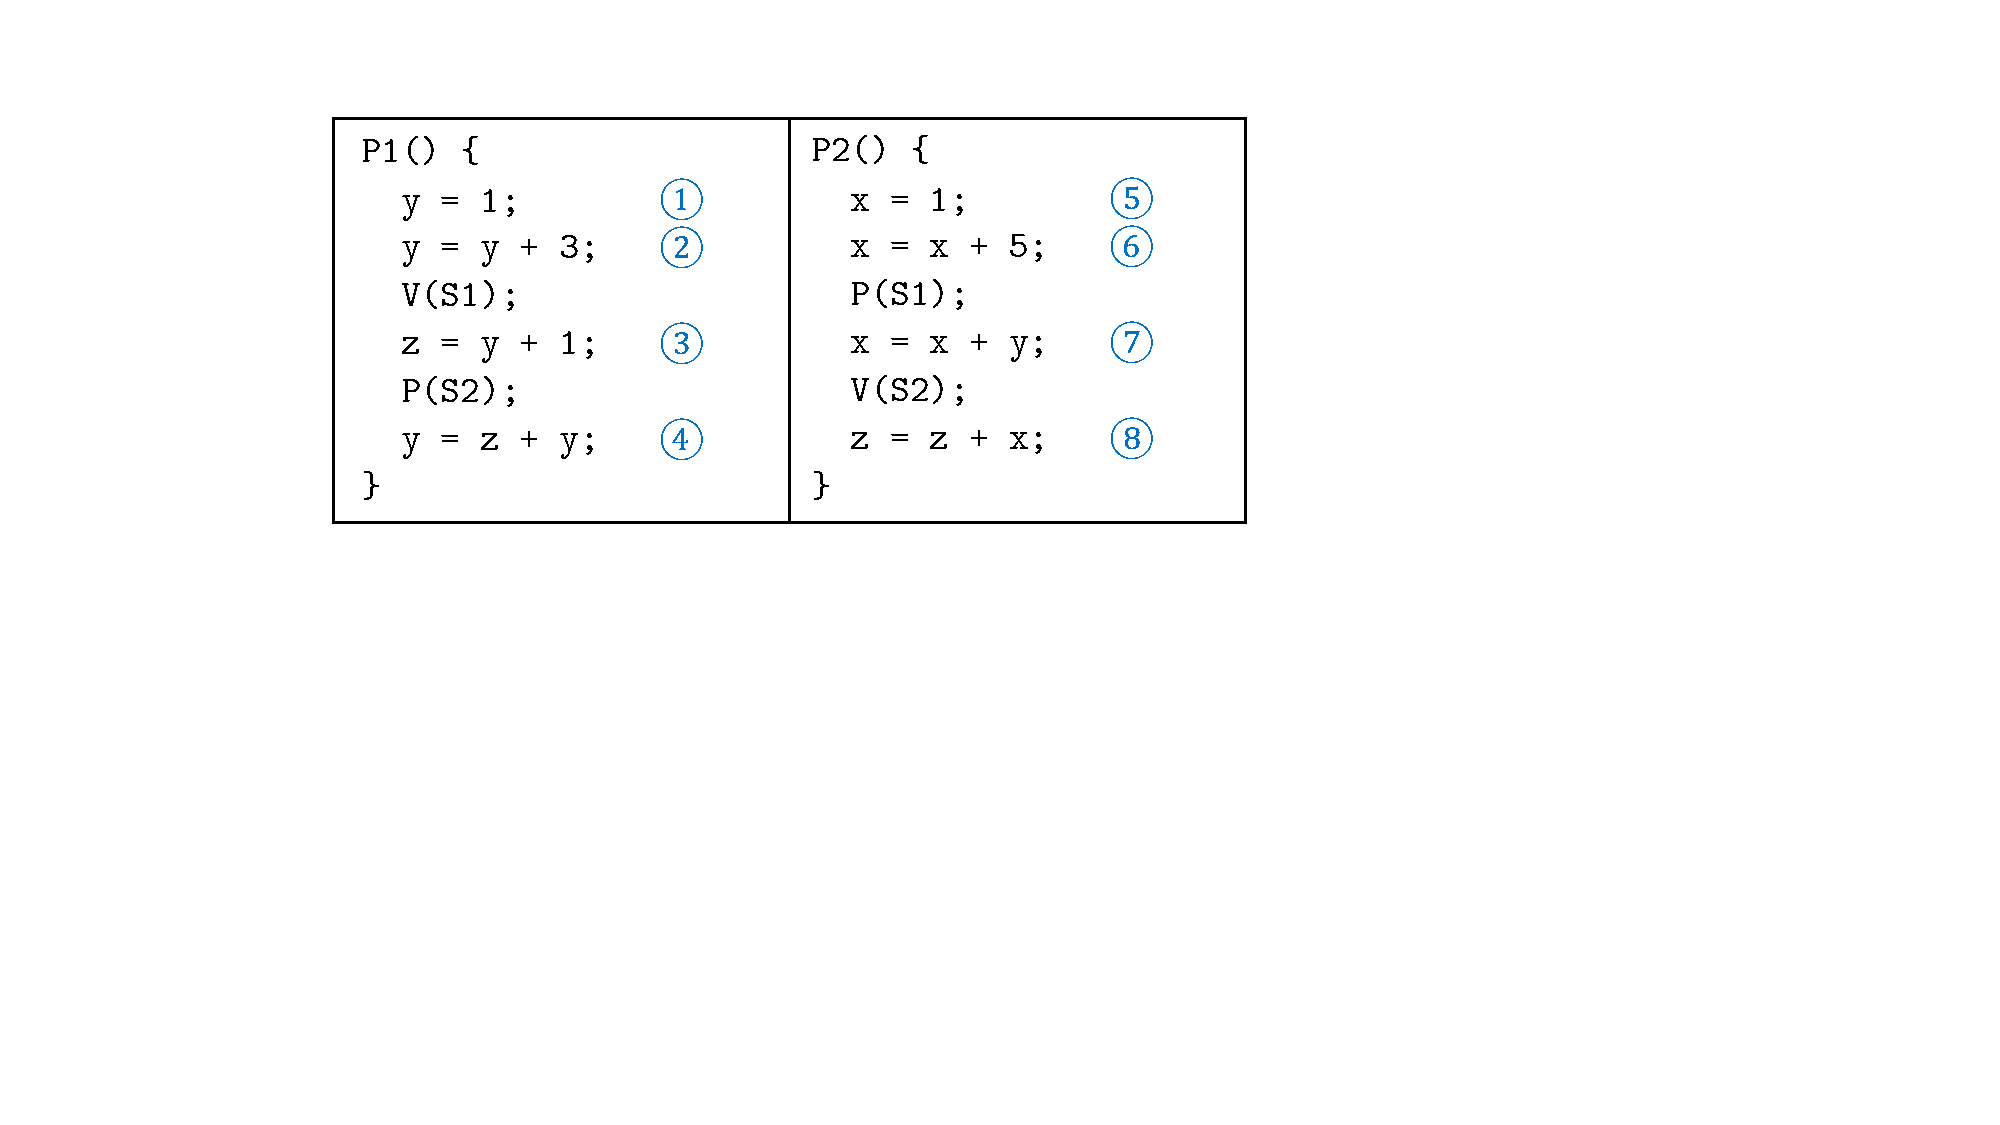
\includegraphics[width=0.46\linewidth]{img/5.pdf}
		\vspace{-1.5em}
	\end{figure}
	\ding{172}、\ding{173}、\ding{176}和\ding{177}是不相交语句,可以任何次序交错执行,而结果是唯一的。接着无论系统如何调度进程并发执行,当执行到语句\ding{178}时,可以得到$x=10,y=4$。按 Bernstein条件,语句\ding{174}的执行结果不受语句\ding{178}的影响,故语句\ding{174}执行后得到$z=5$。最后,语句\ding{175}和\ding{179}并发执行,这时得到了两种结果为:

	语句\ding{175}先执行(即执行顺序为\ding{174}、\ding{178}、\ding{175}、\ding{179})的结果为$x=10, y=9, z=15$。
	
	语句\ding{179}先执行(即执行顺序为\ding{174}、\ding{178}、\ding{179}、\ding{175})的结果为$x=10, y=19, z=15$。

	此外,还有第三种情况,语句\ding{174}被推迟,直至语句\ding{179}后再执行,即执行顺序为\ding{178}、\ding{179}、\ding{174}、\ding{175}。
	这时$z$的值只可能是$y+1=5$,故$y=z+y=5+4=9$,而$x=10$。

	即第三种情况的结果为$x=10,y=9,z=5$。
\end{solution}


\begin{problem}
	四个进程$P_i(i=0,\cdots,3)$和四个信箱$M_j(j=0,\cdots,3)$,进程间借助相邻信箱传递消息,即$P_i$每次从$M_i$中取一条消息,经加工后送入$M(i+1) \mod 4$,其中$M_0$、$M_1$、$M_2$、$M_3$分别可存放3、3、2、2个消息。初始状态下,$M_0$装了三条消息,其余为空。试以P、V操作为工具,写出$P_i(i=0,\cdots,3)$的同步工作算法。
	\begin{figure}[H]
		\centering
		\vspace{-0.5em}
		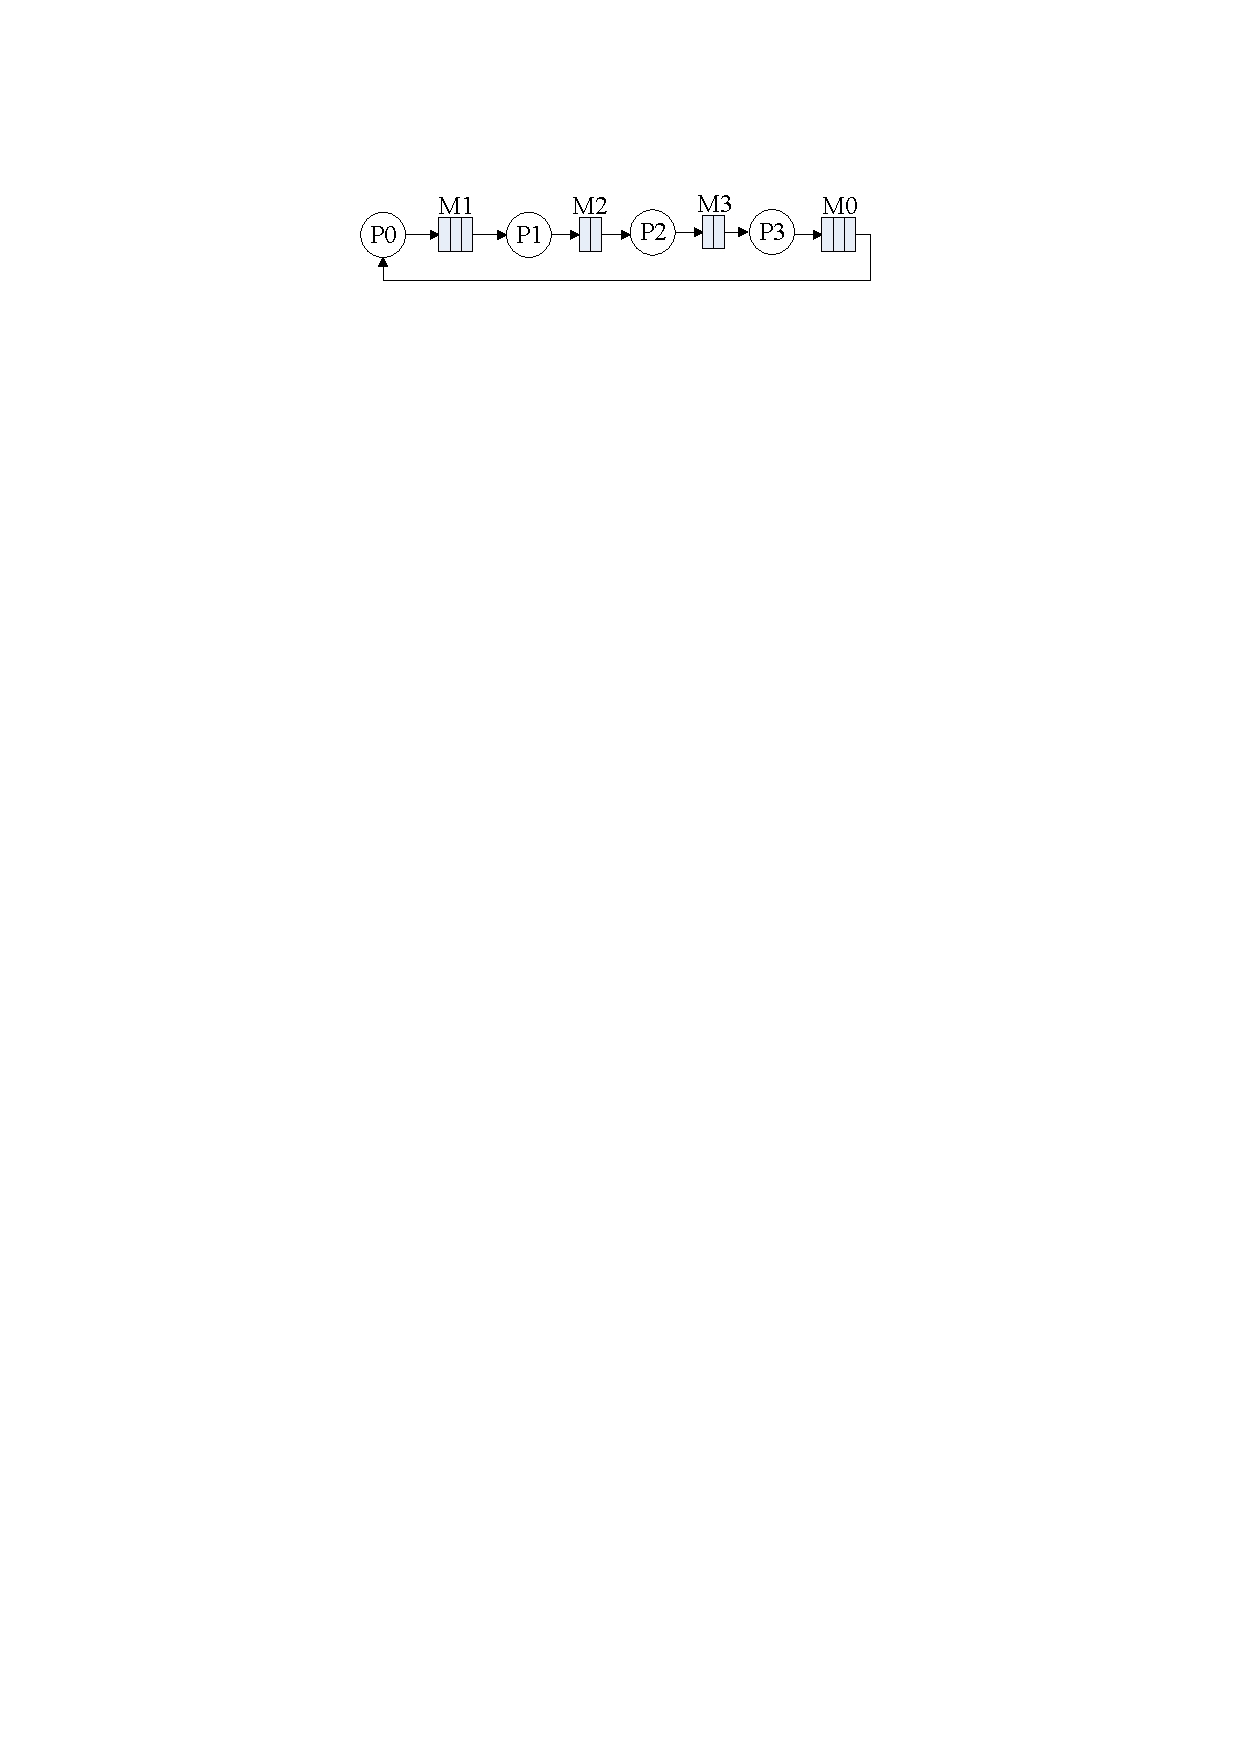
\includegraphics[width=0.45\linewidth]{img/6.pdf}
		\vspace{-1em}
	\end{figure}
\end{problem}

\begin{solution}
	\begin{figure}[H]
		\centering
		\vspace{-2em}
		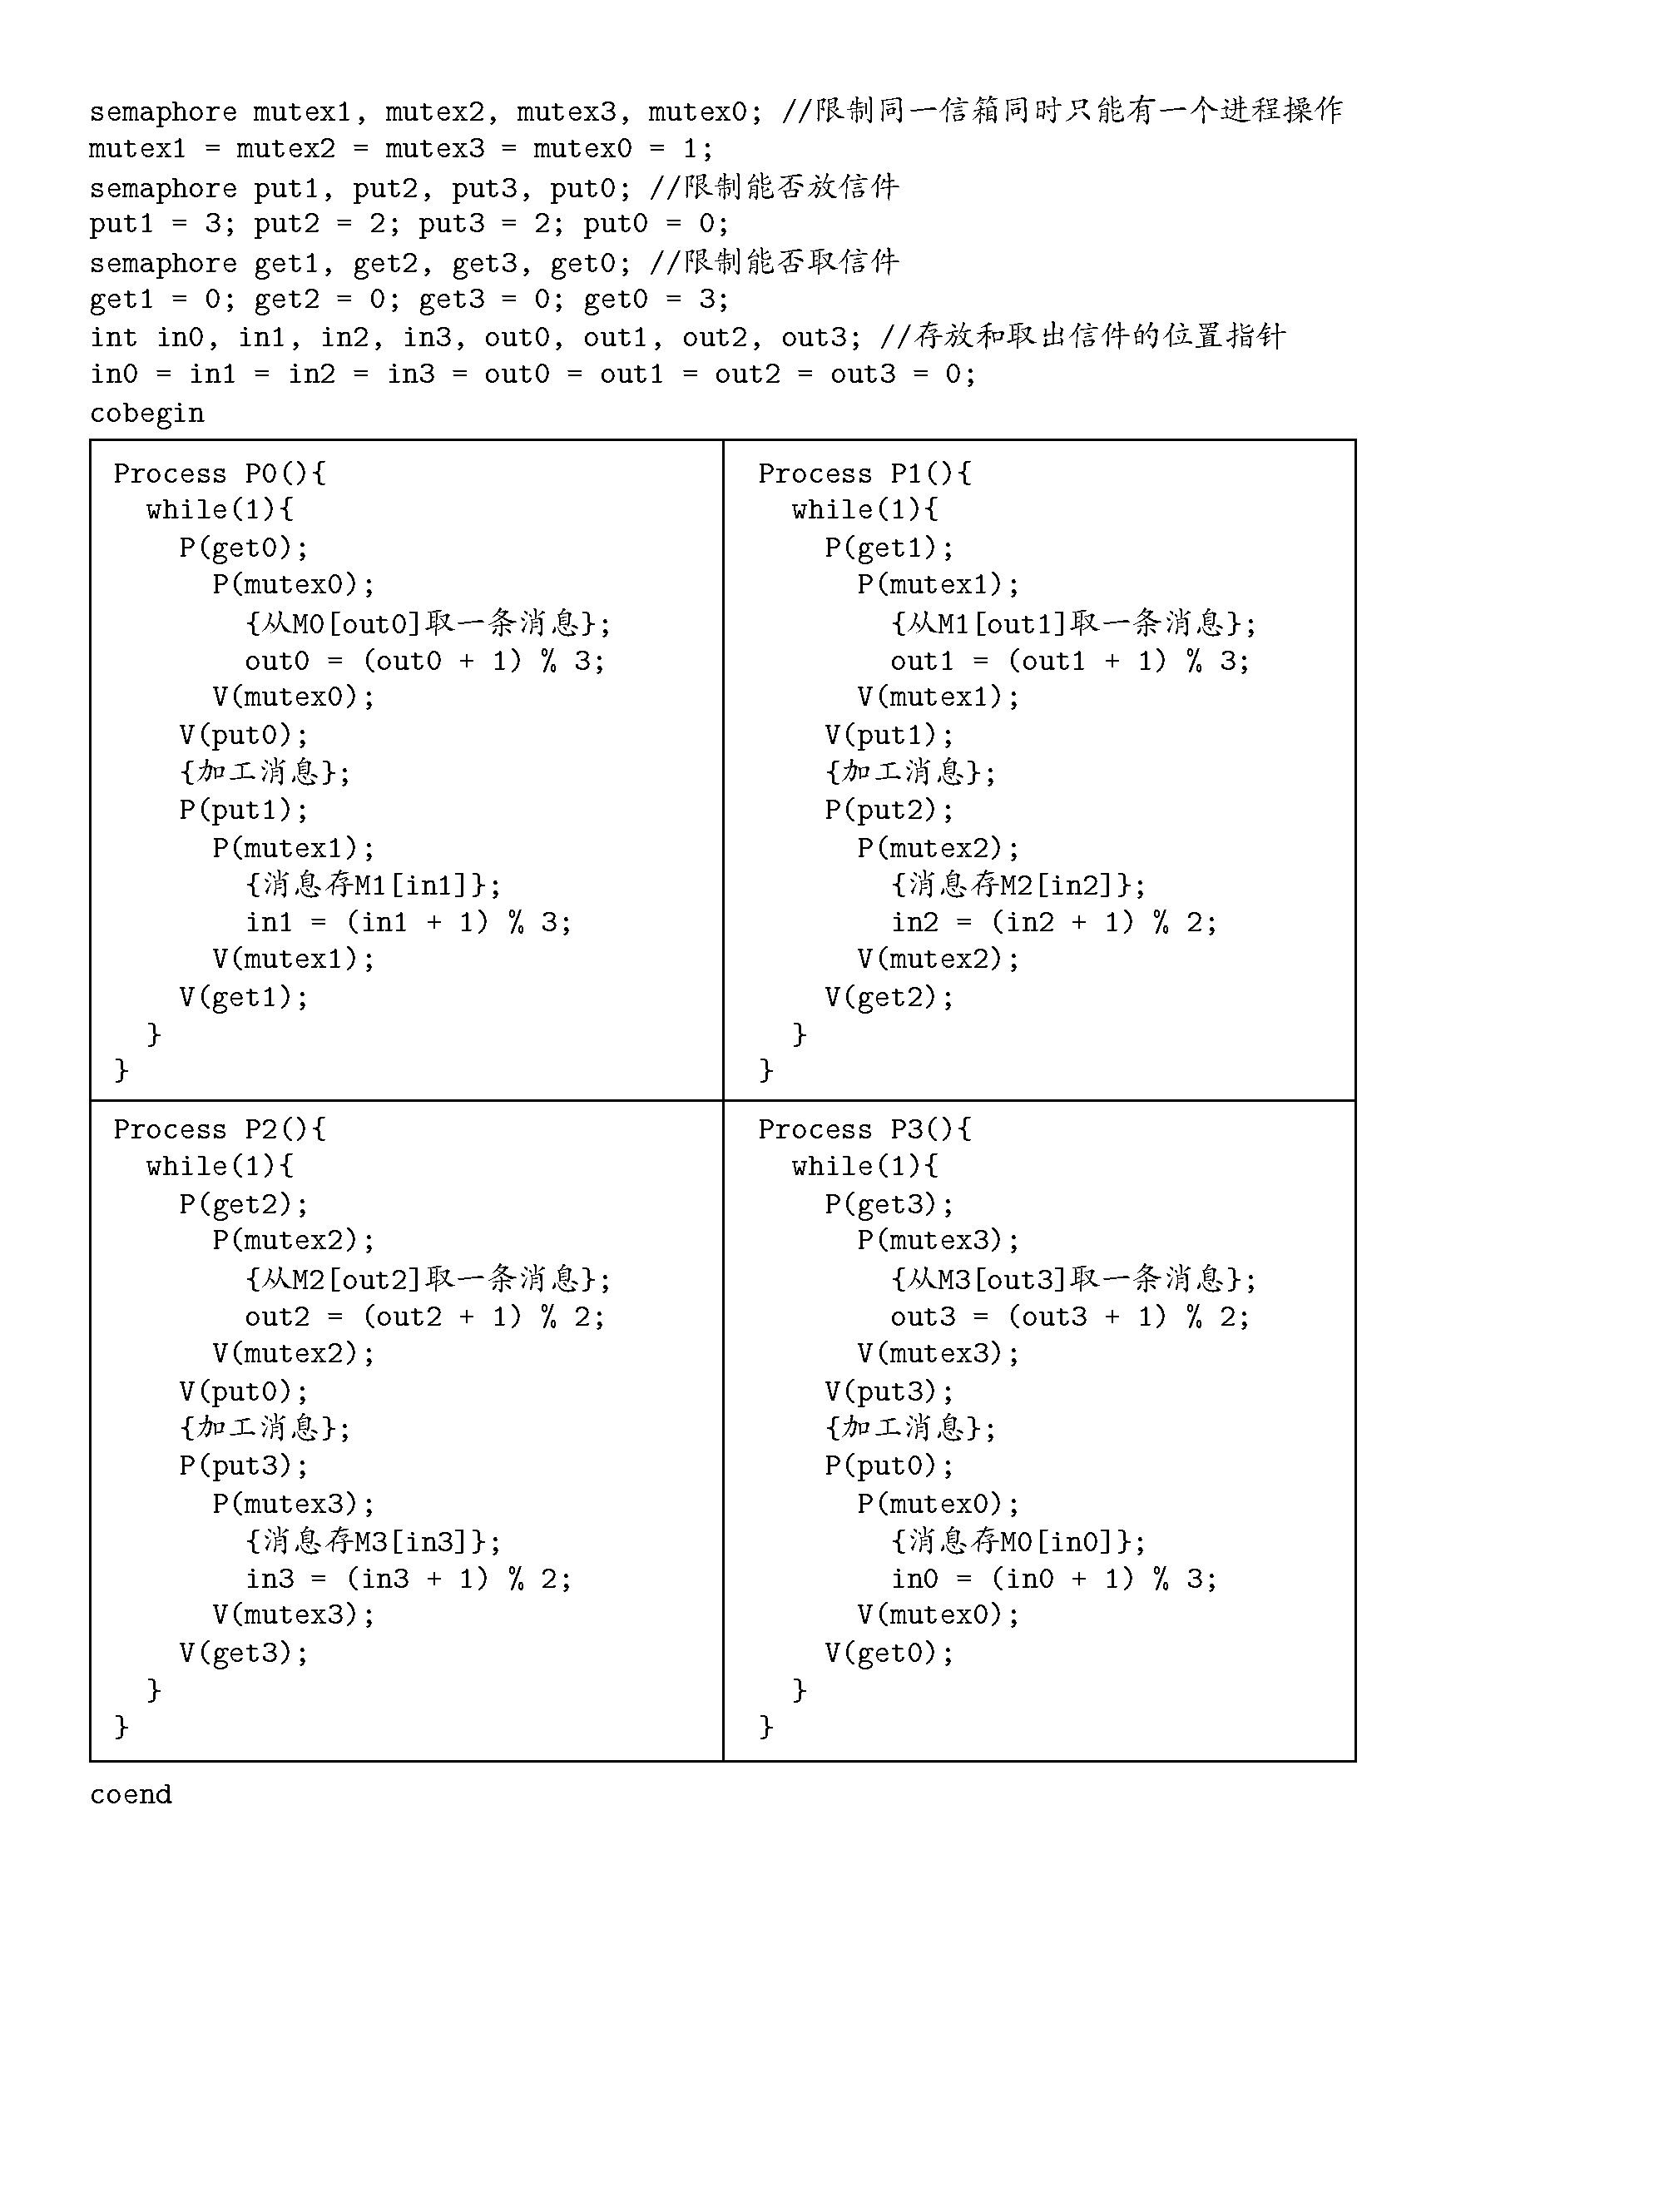
\includegraphics[width=0.89\linewidth]{img/6.1.pdf}
		\vspace{-1em}
	\end{figure}
\end{solution}


\begin{problem}
	有一个阅览室,读者进入时必须先在一张登记表上登记,此表为每个座位列出一个表目,包括座位号、姓名,读者离开时要注销登记信息;假如阅览室共有100个座位。试用:(1)信号量和PV操作;(2)管程,实现用户进程的同步算法。
\end{problem}

\begin{solution}
	(1)使用信号量和PV操作
	\begin{figure}[H]
		\centering
		\vspace{-0.5em}
		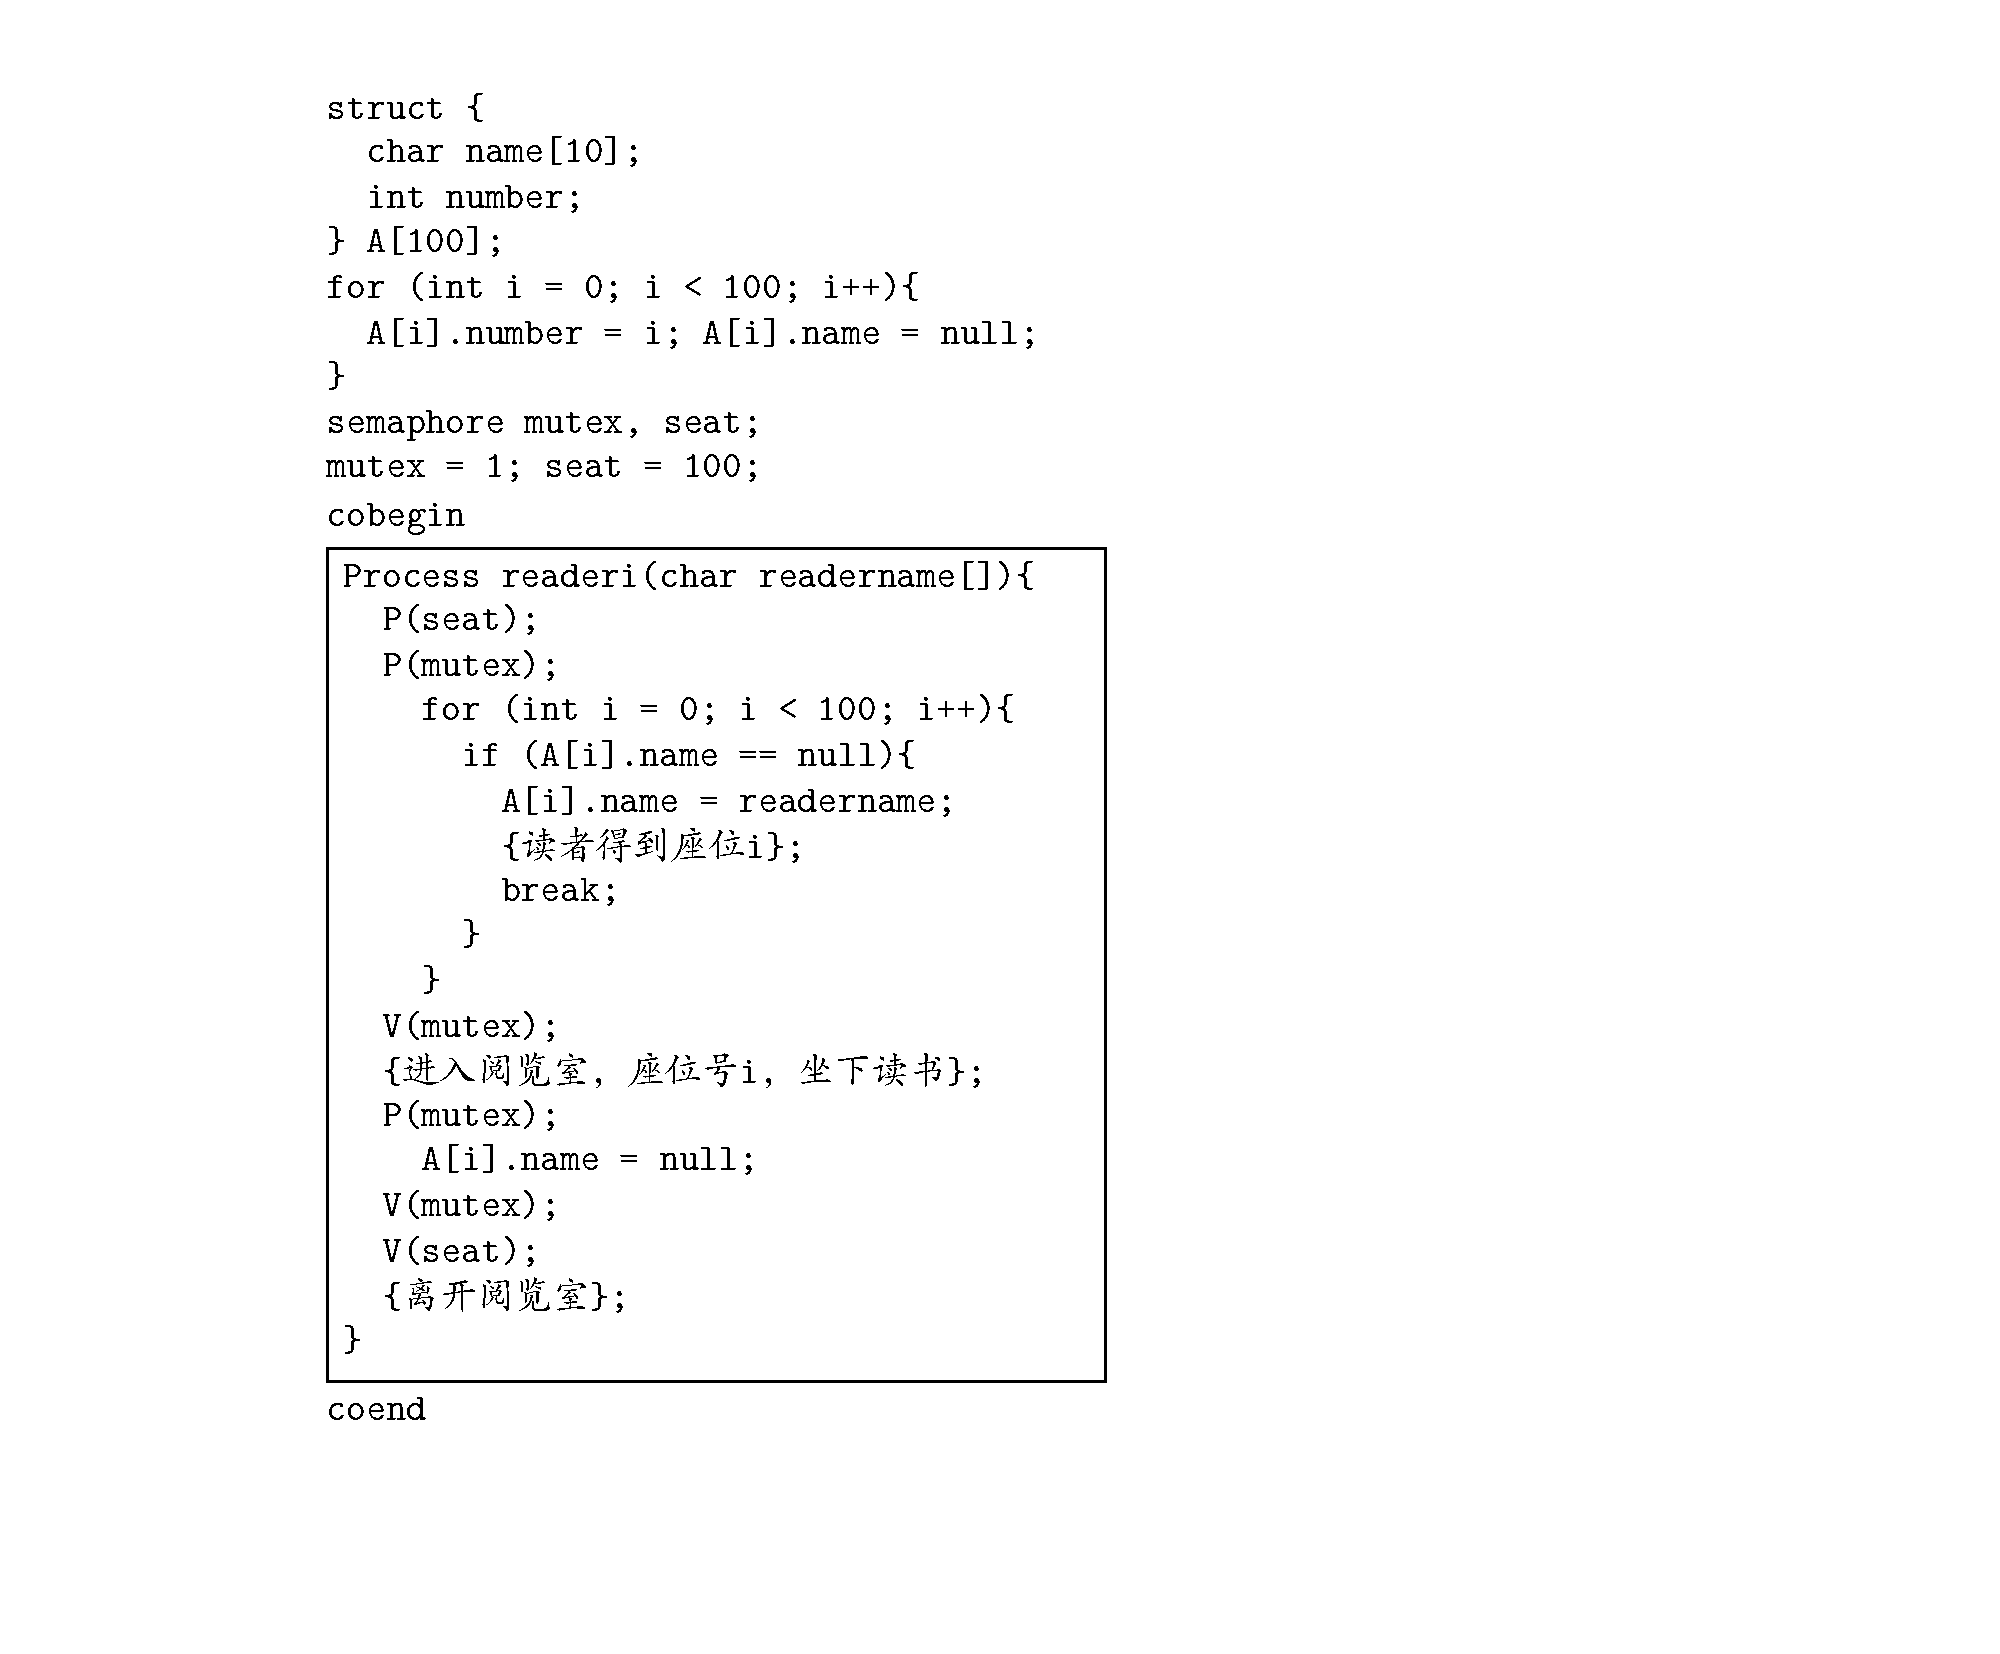
\includegraphics[width=0.35\linewidth]{img/7.1.pdf}
		\vspace{-1em}
	\end{figure}
	(2)使用管程实现
	\begin{figure}[H]
		\centering
		\vspace{-0.5em}
		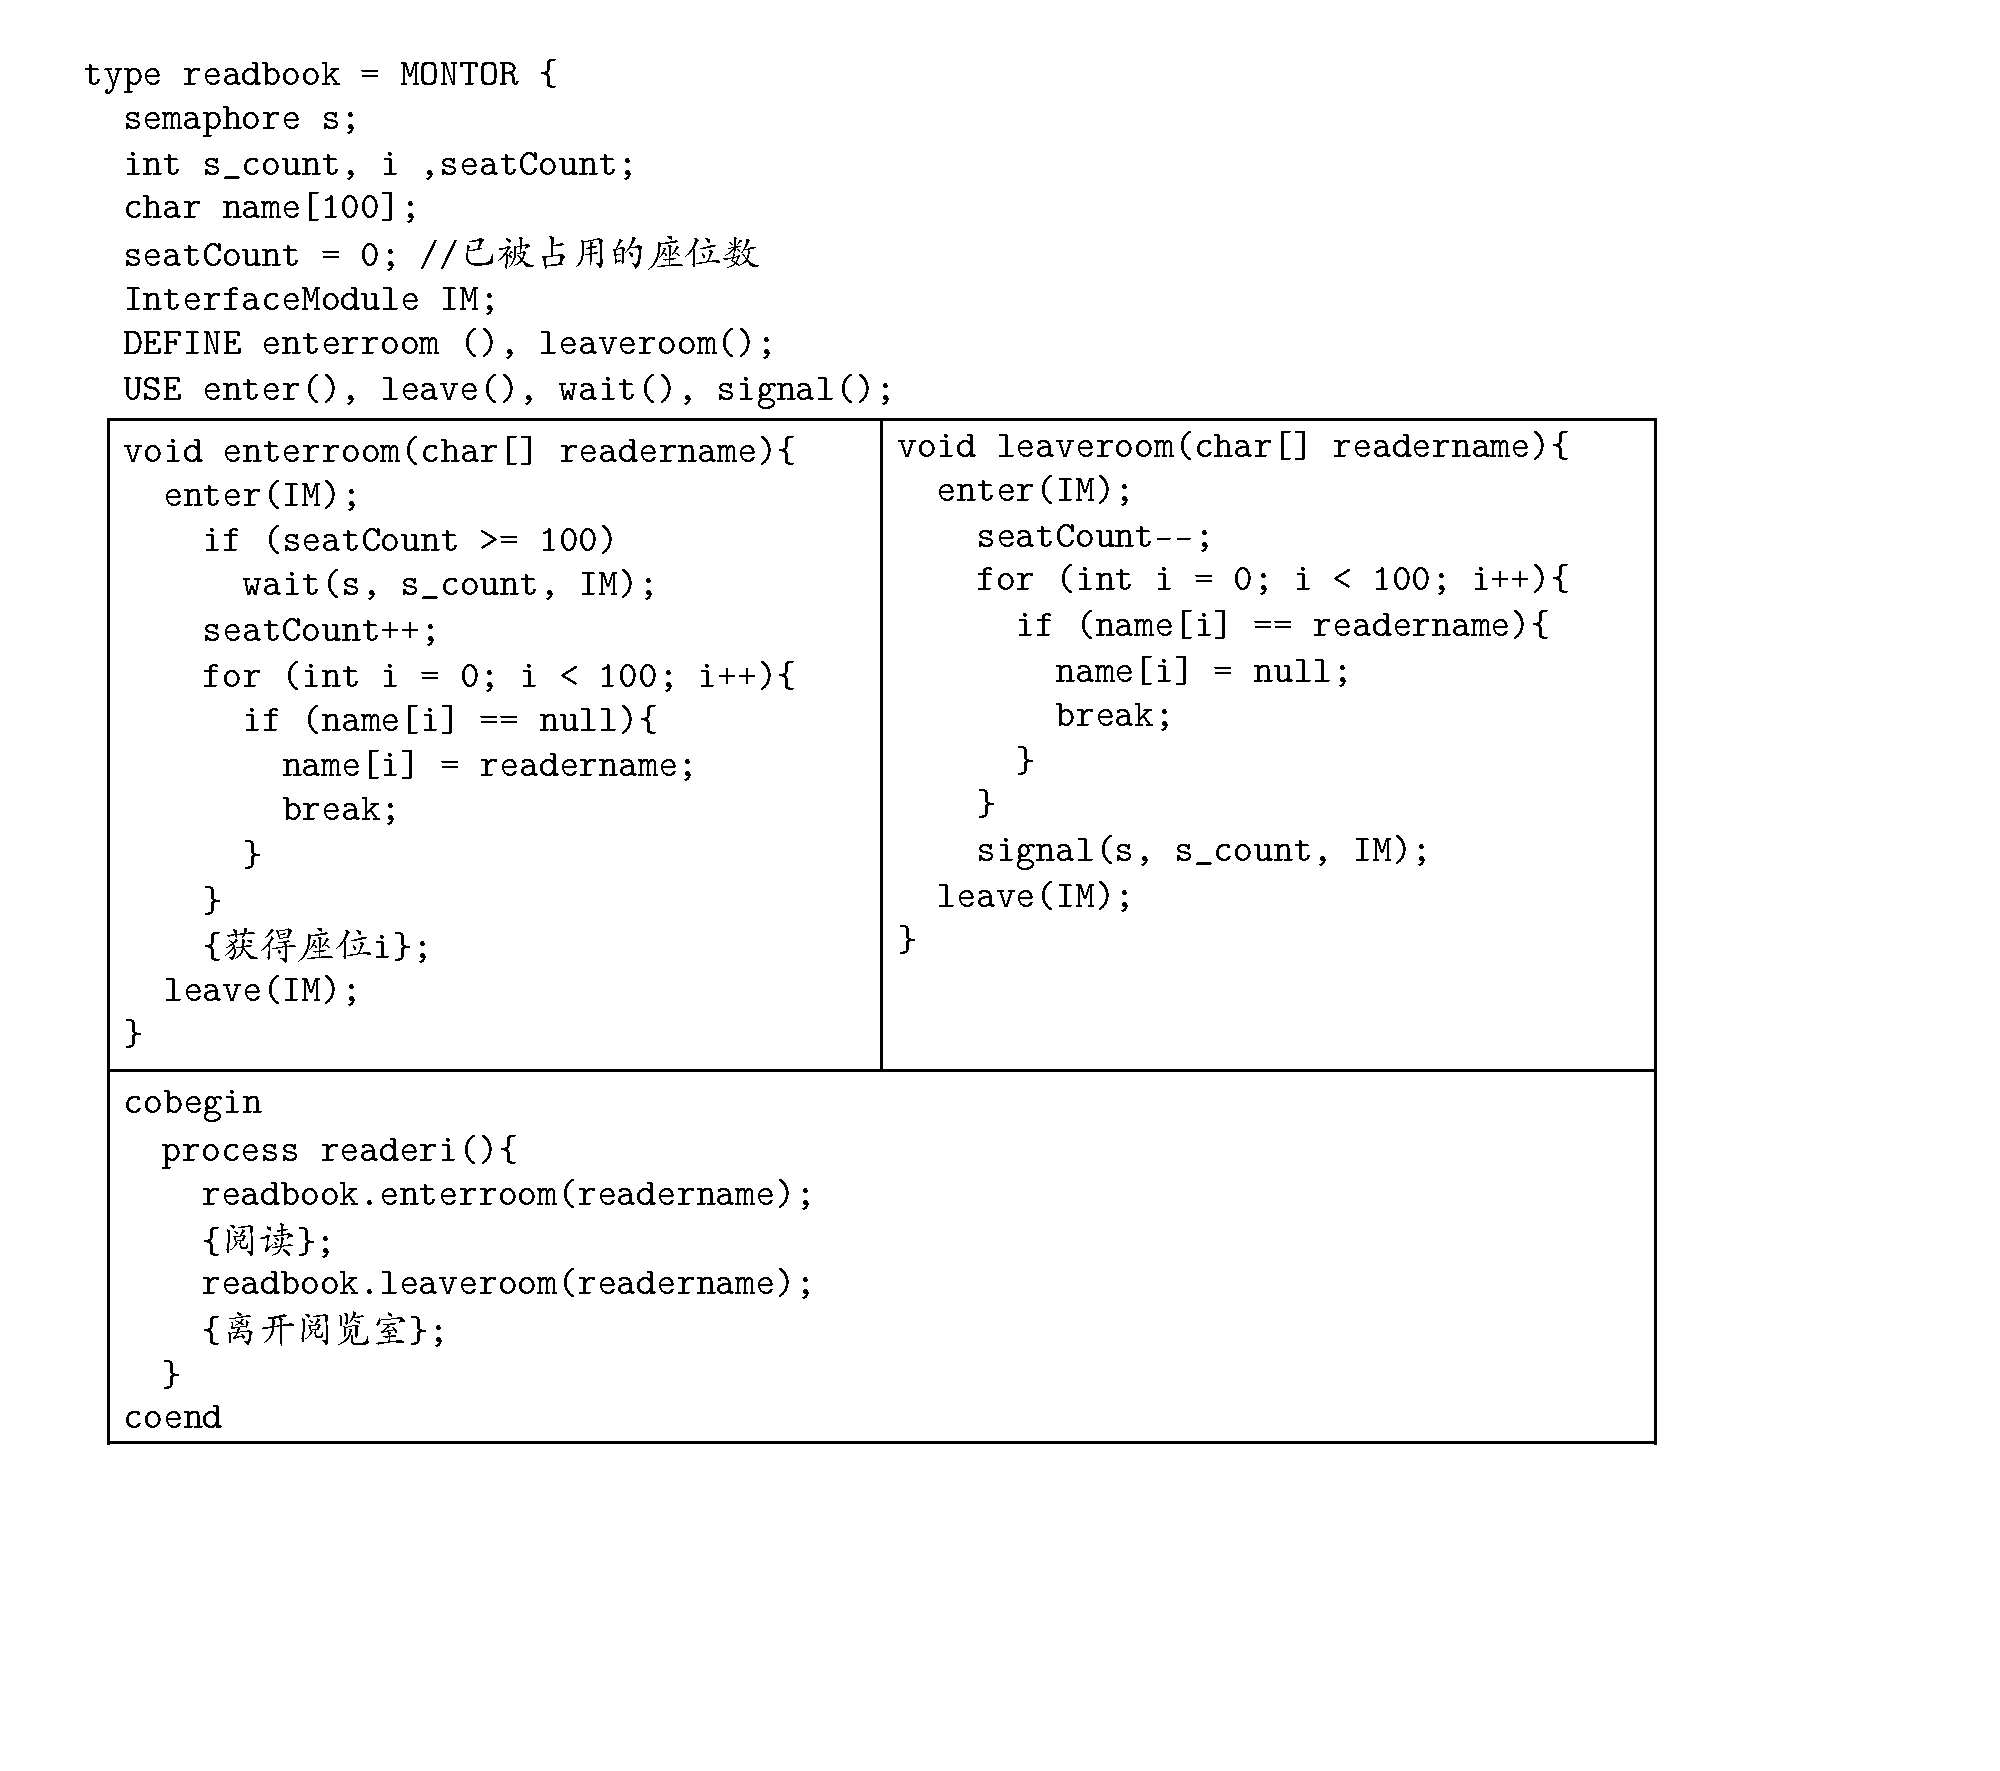
\includegraphics[width=0.72\linewidth]{img/7.2.pdf}
		\vspace{-1em}
	\end{figure}
\end{solution}


\begin{problem}
	在一个盒子里,混装了数量相等的黑白围棋子。现在用自动分拣系统把黑子、白子分开,设分拣系统有二个进程$P_1$和$P_2$,其中$P_1$拣白子;$P_2$拣黑子。规定每个进程每次拣一子;当一个进程在拣时,不允许另一个进程去拣;当一个进程拣了一子时,必须让另一个进程去拣。试分别使用(1)\;PV操作和(2)管程方法写出两进程$P_1$和$P_2$能并发正确执行的程序。
\end{problem}

\begin{solution}
	(1)使用信号量和PV操作
	\begin{figure}[H]
		\centering
		\vspace{-0.5em}
		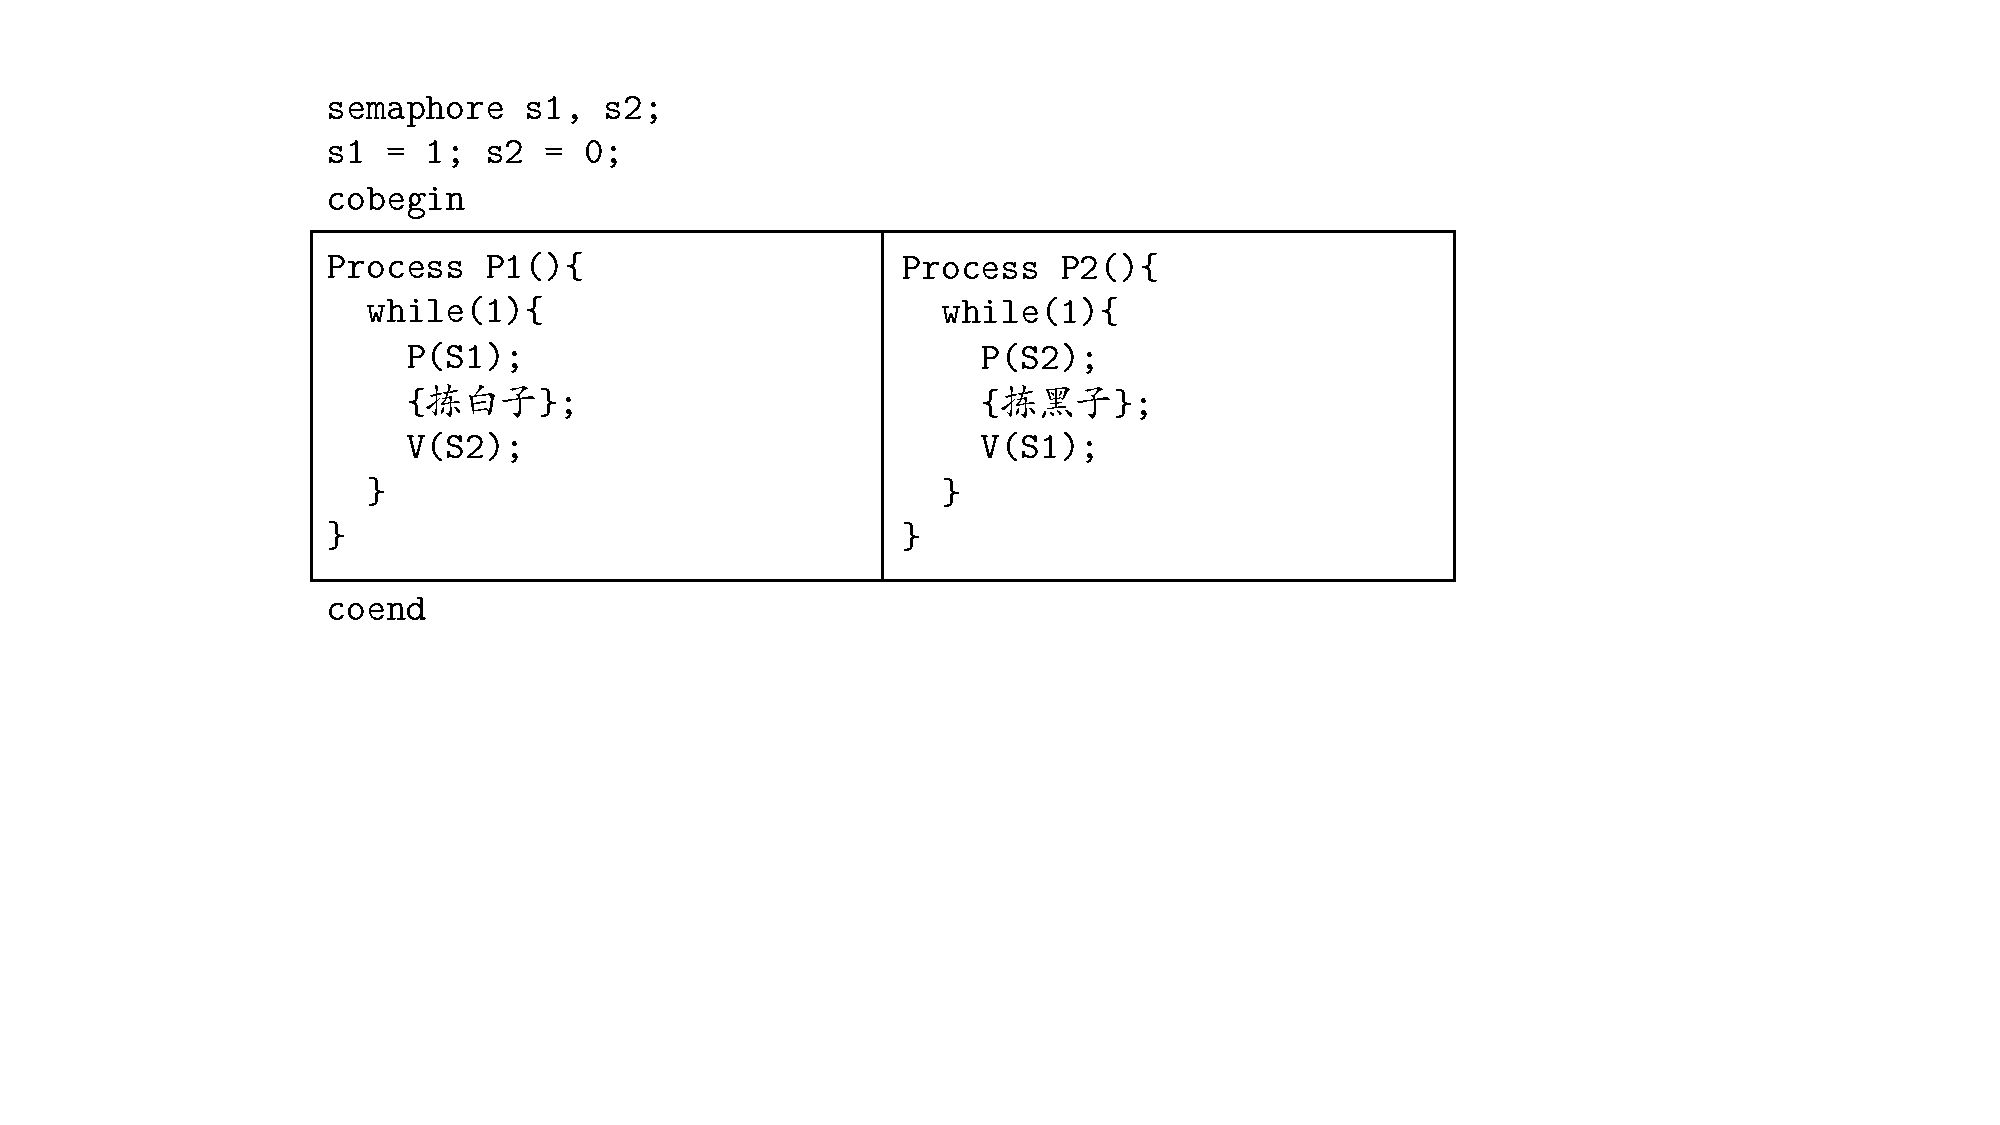
\includegraphics[width=0.7\linewidth]{img/8.1.pdf}
		\vspace{-1em}
	\end{figure}
	(2)使用管程实现
	\begin{figure}[H]
		\centering
		\vspace{-0.5em}
		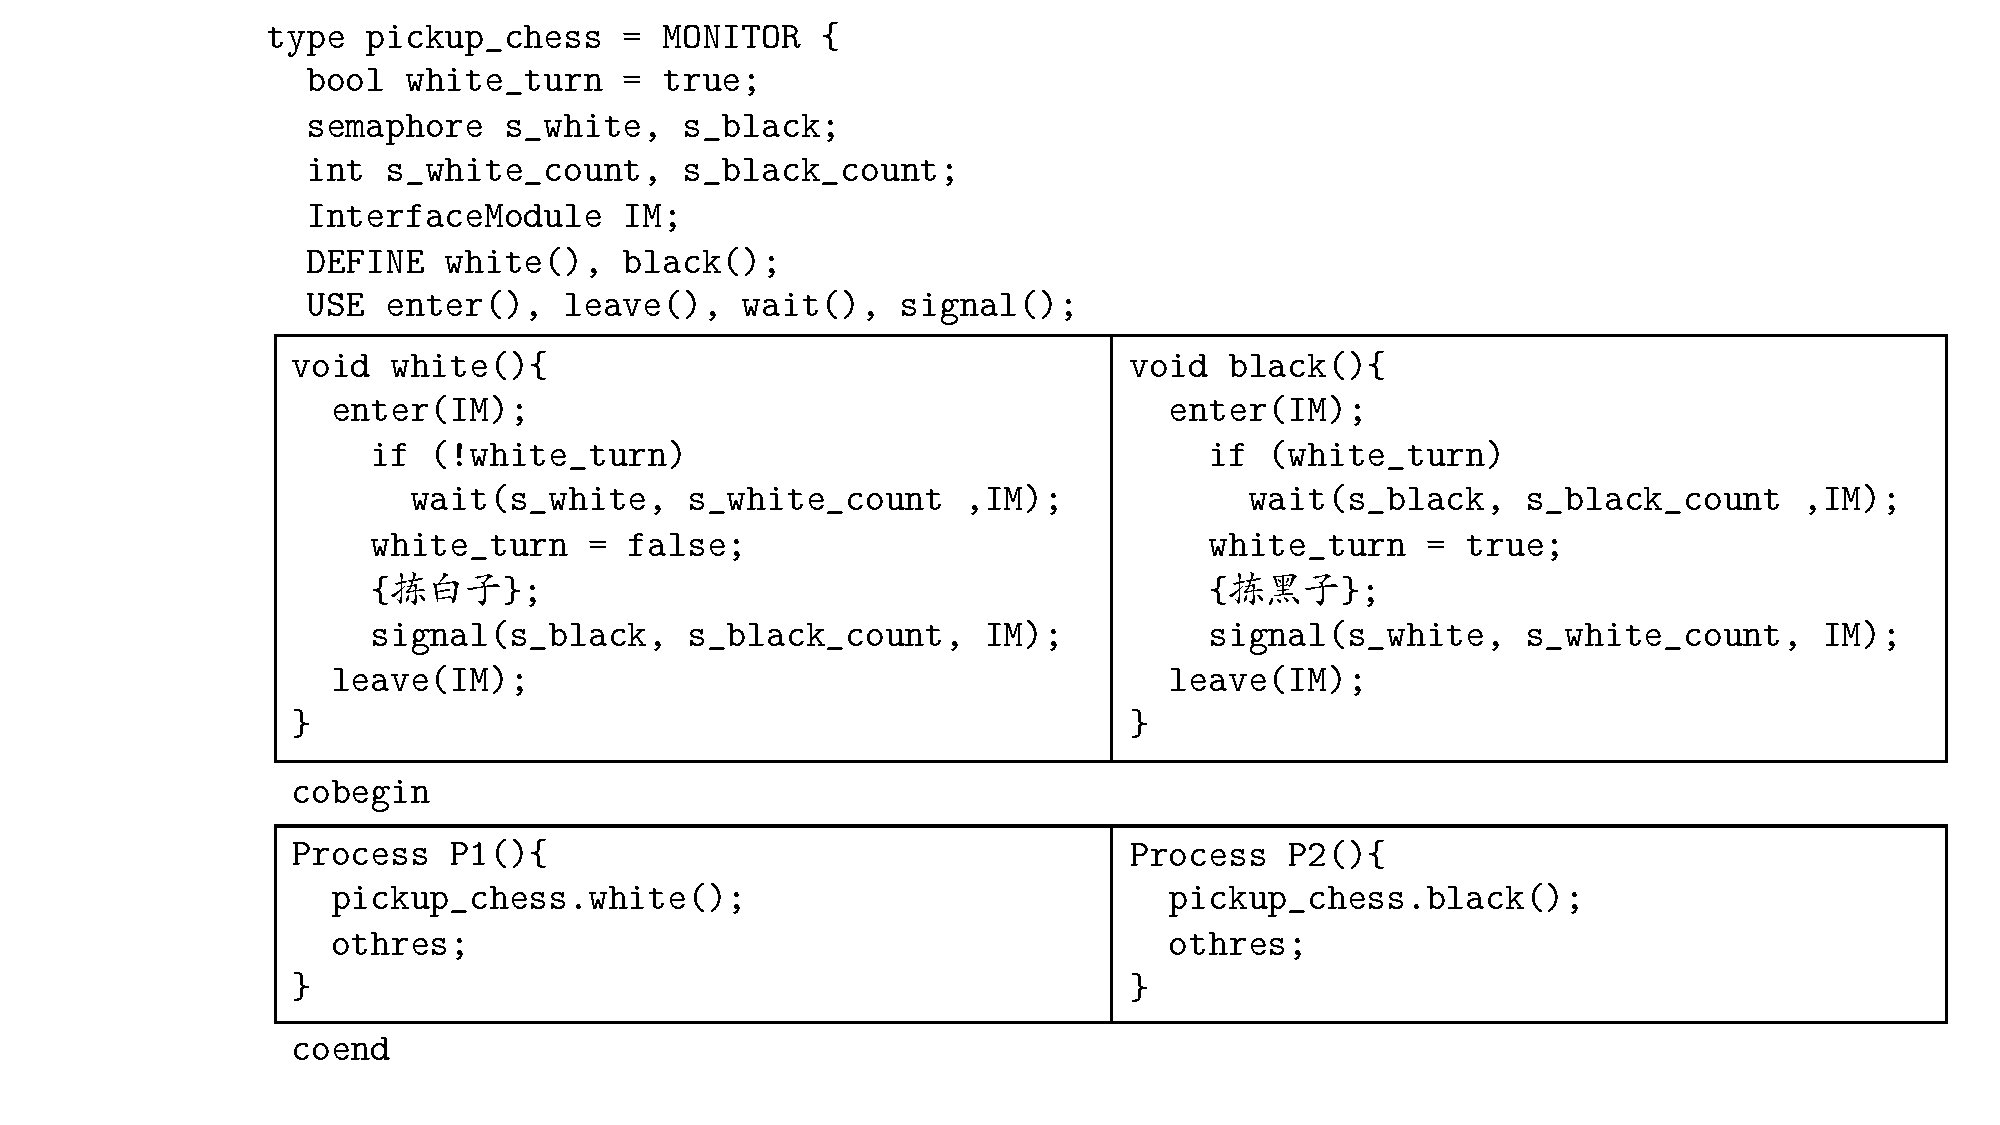
\includegraphics[width=0.95\linewidth]{img/8.2.pdf}
		\vspace{-1em}
	\end{figure}
\end{solution}

\clearpage

\begin{problem}
	一组生产者进程和一组消费者进程共享9个缓冲区,每个缓冲区可以存放一个整数。生产者进程每次一次性地向3个缓冲区中写入整数,消费者进程每次从缓冲区取出一个整数。请用:(1)信号量和PV操作;(2)管程方法写出能够正确执行的程序。
\end{problem}

\begin{solution}
	(1)使用信号量和PV操作
	\begin{figure}[H]
		\centering
		\vspace{-0.5em}
		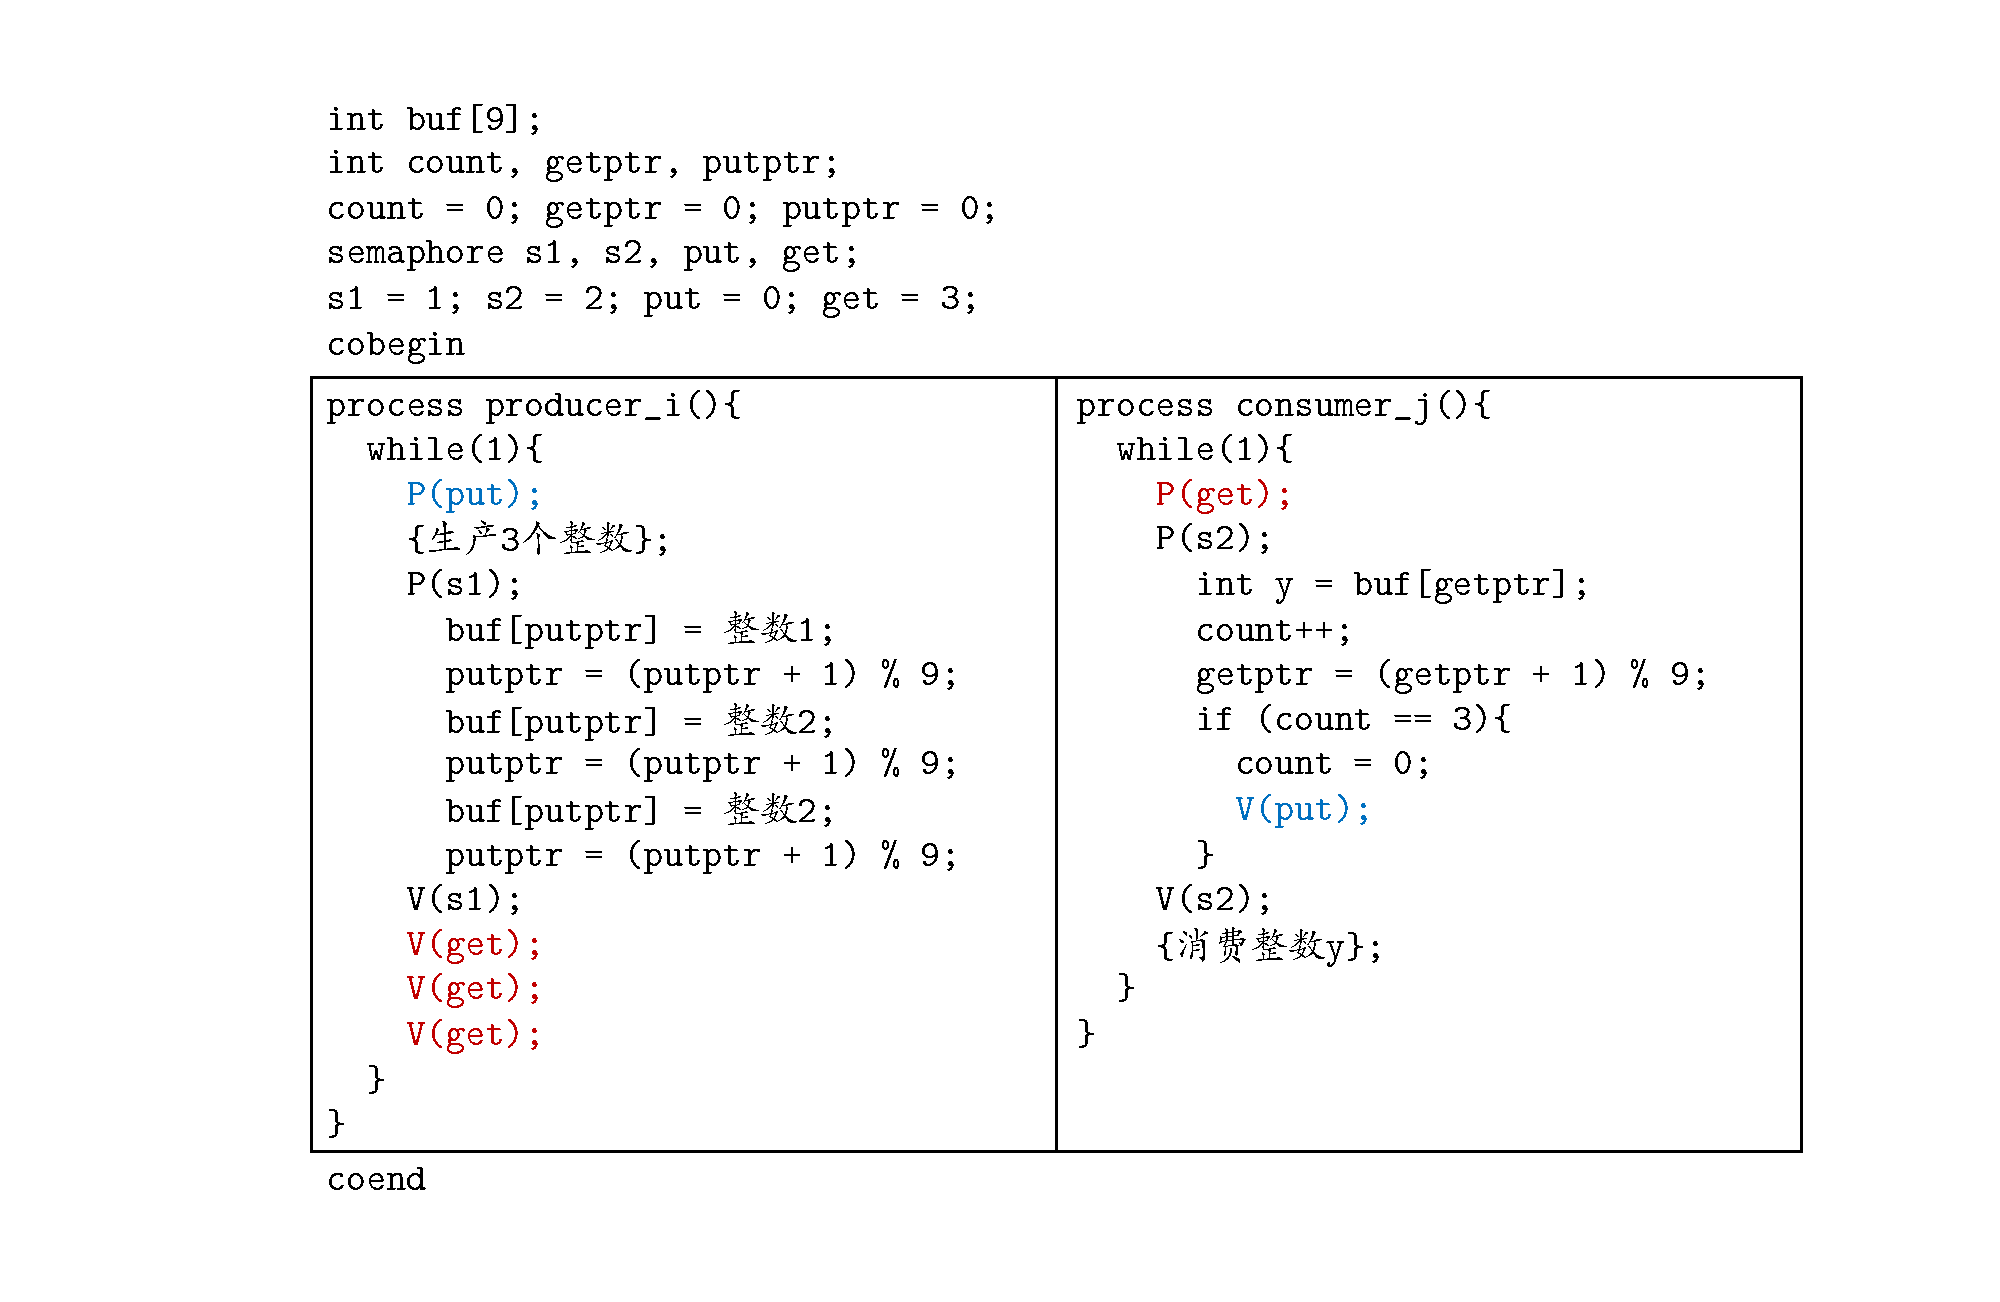
\includegraphics[width=0.7\linewidth]{img/9.1.pdf}
		\vspace{-1em}
	\end{figure}
	(2)使用管程实现
	\begin{figure}[H]
		\centering
		\vspace{-0.5em}
		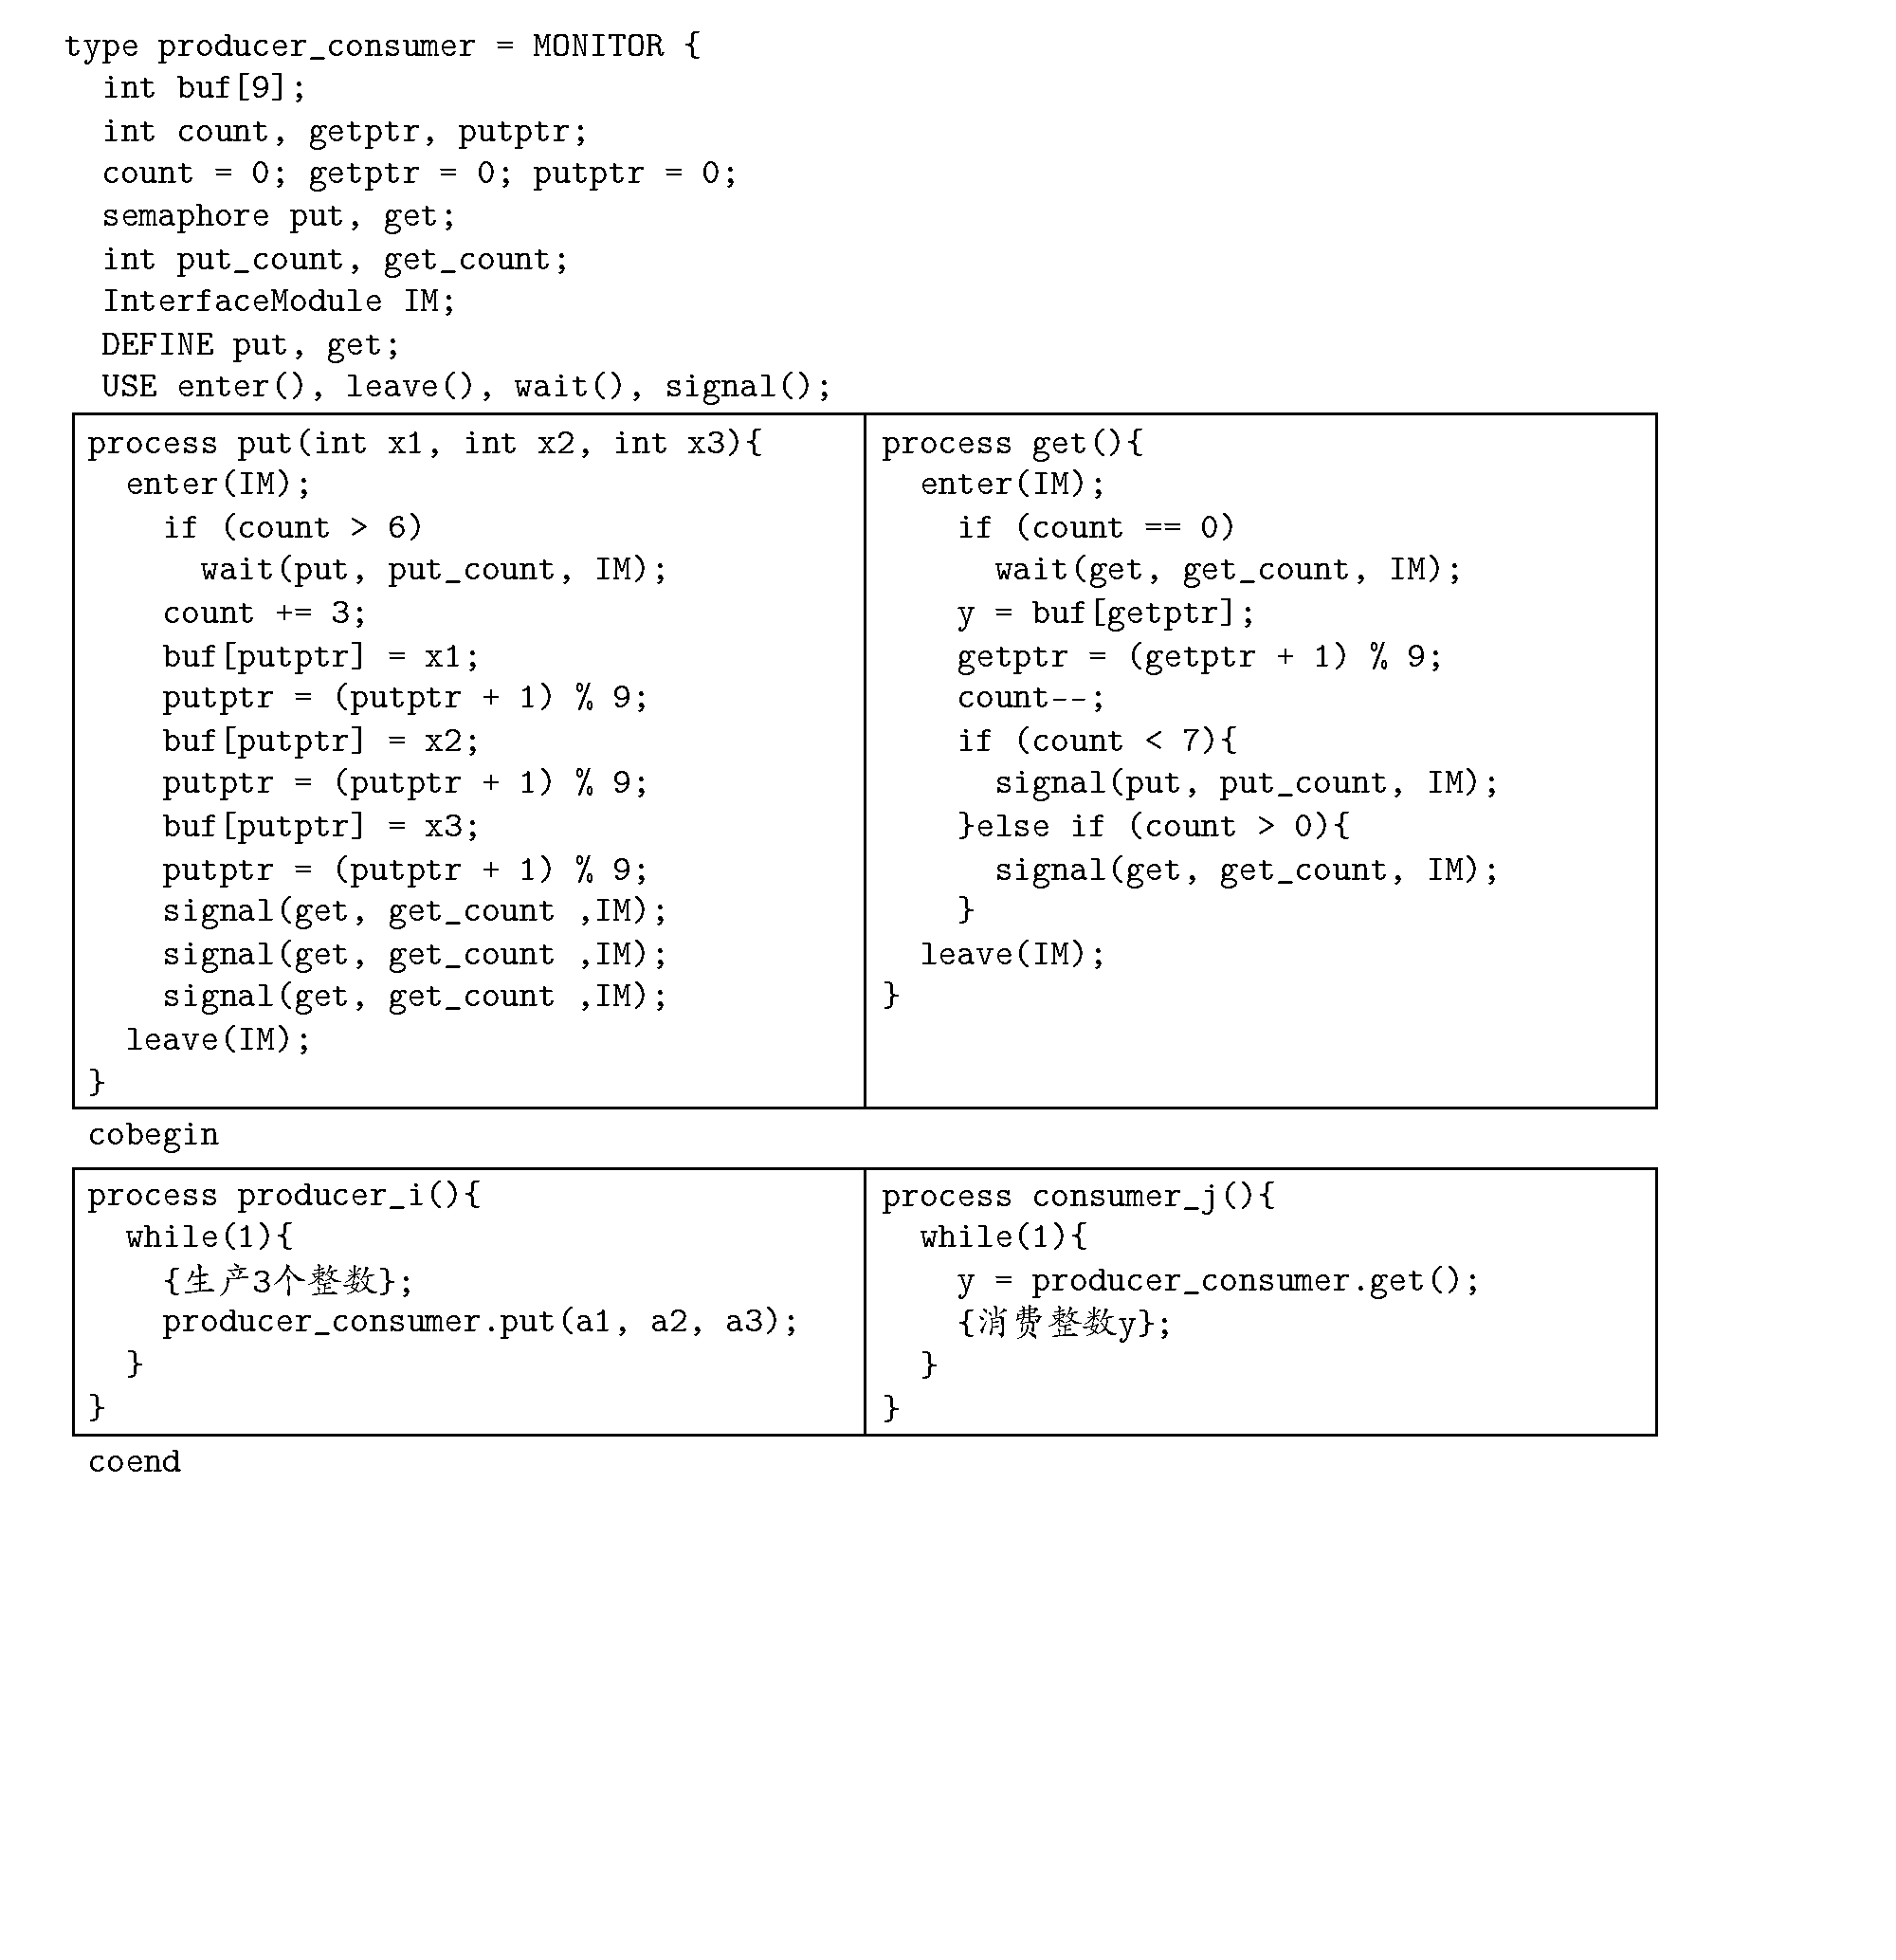
\includegraphics[width=0.79\linewidth]{img/9.2.pdf}
		\vspace{-1em}
	\end{figure}
\end{solution}


\begin{problem}
	系统有$A,B,C,D$共4种资源,在某时刻进程$P_0,P_1,P_2,P_3$和$P_4$对资源的占有和需求情况如表,试解答下列问题:
	\begin{figure}[H]
		\centering
		\vspace{-0.5em}
		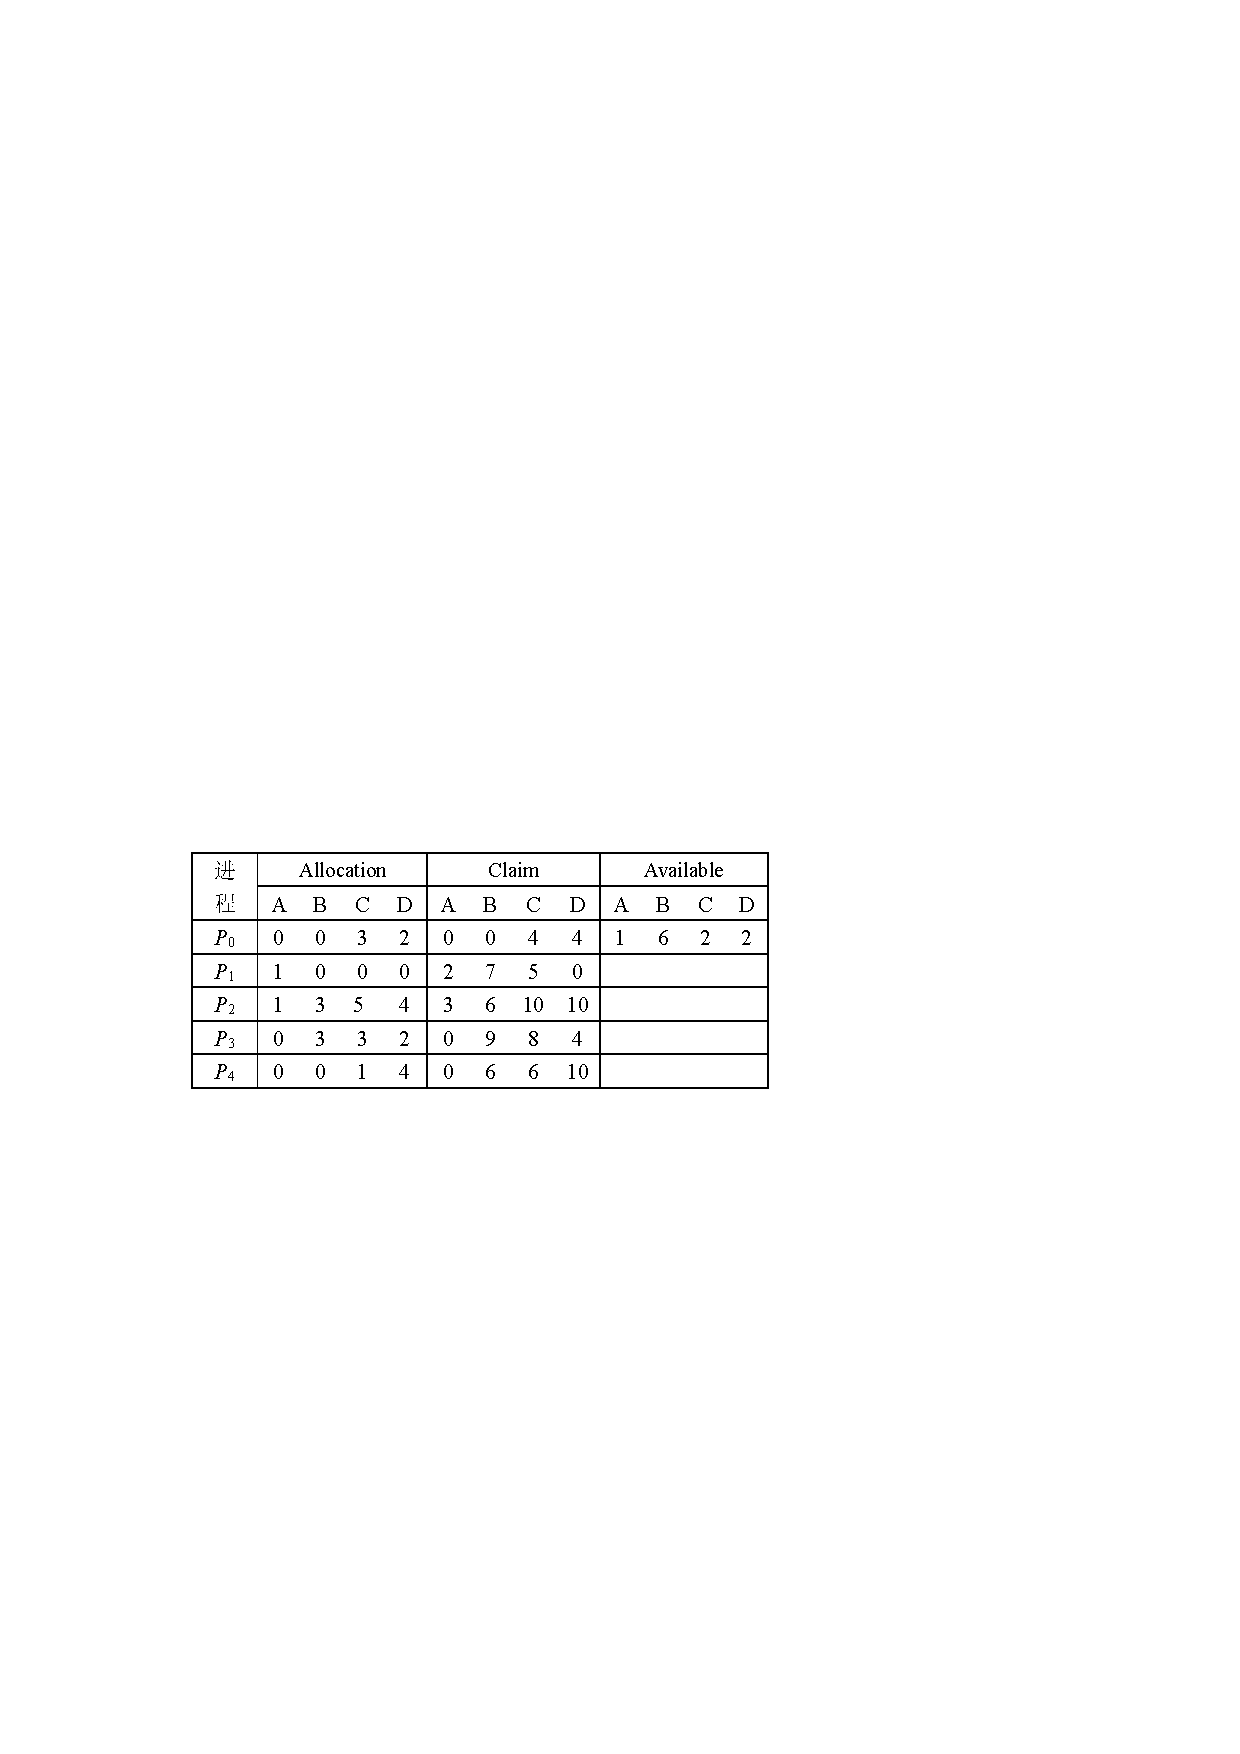
\includegraphics[width=0.6\linewidth]{img/10.1.pdf}
		\vspace{-1em}
	\end{figure}
	\begin{enumerate}[label=(\arabic*)]
		\item 系统此时处于安全状态吗?试给出一个可能的安全序列。
		\item 若此时进程$P_2$发出$request1(1,2,2,2)$,系统能分配资源给它吗?为什么?
	\end{enumerate}
\end{problem}

\begin{solution}
	(1)系统处于安全状态,一个安全序列为$P_0-P_3-P_4-P_1-P_2$。
	\begin{figure}[H]
		\centering
		\vspace{-0.5em}
		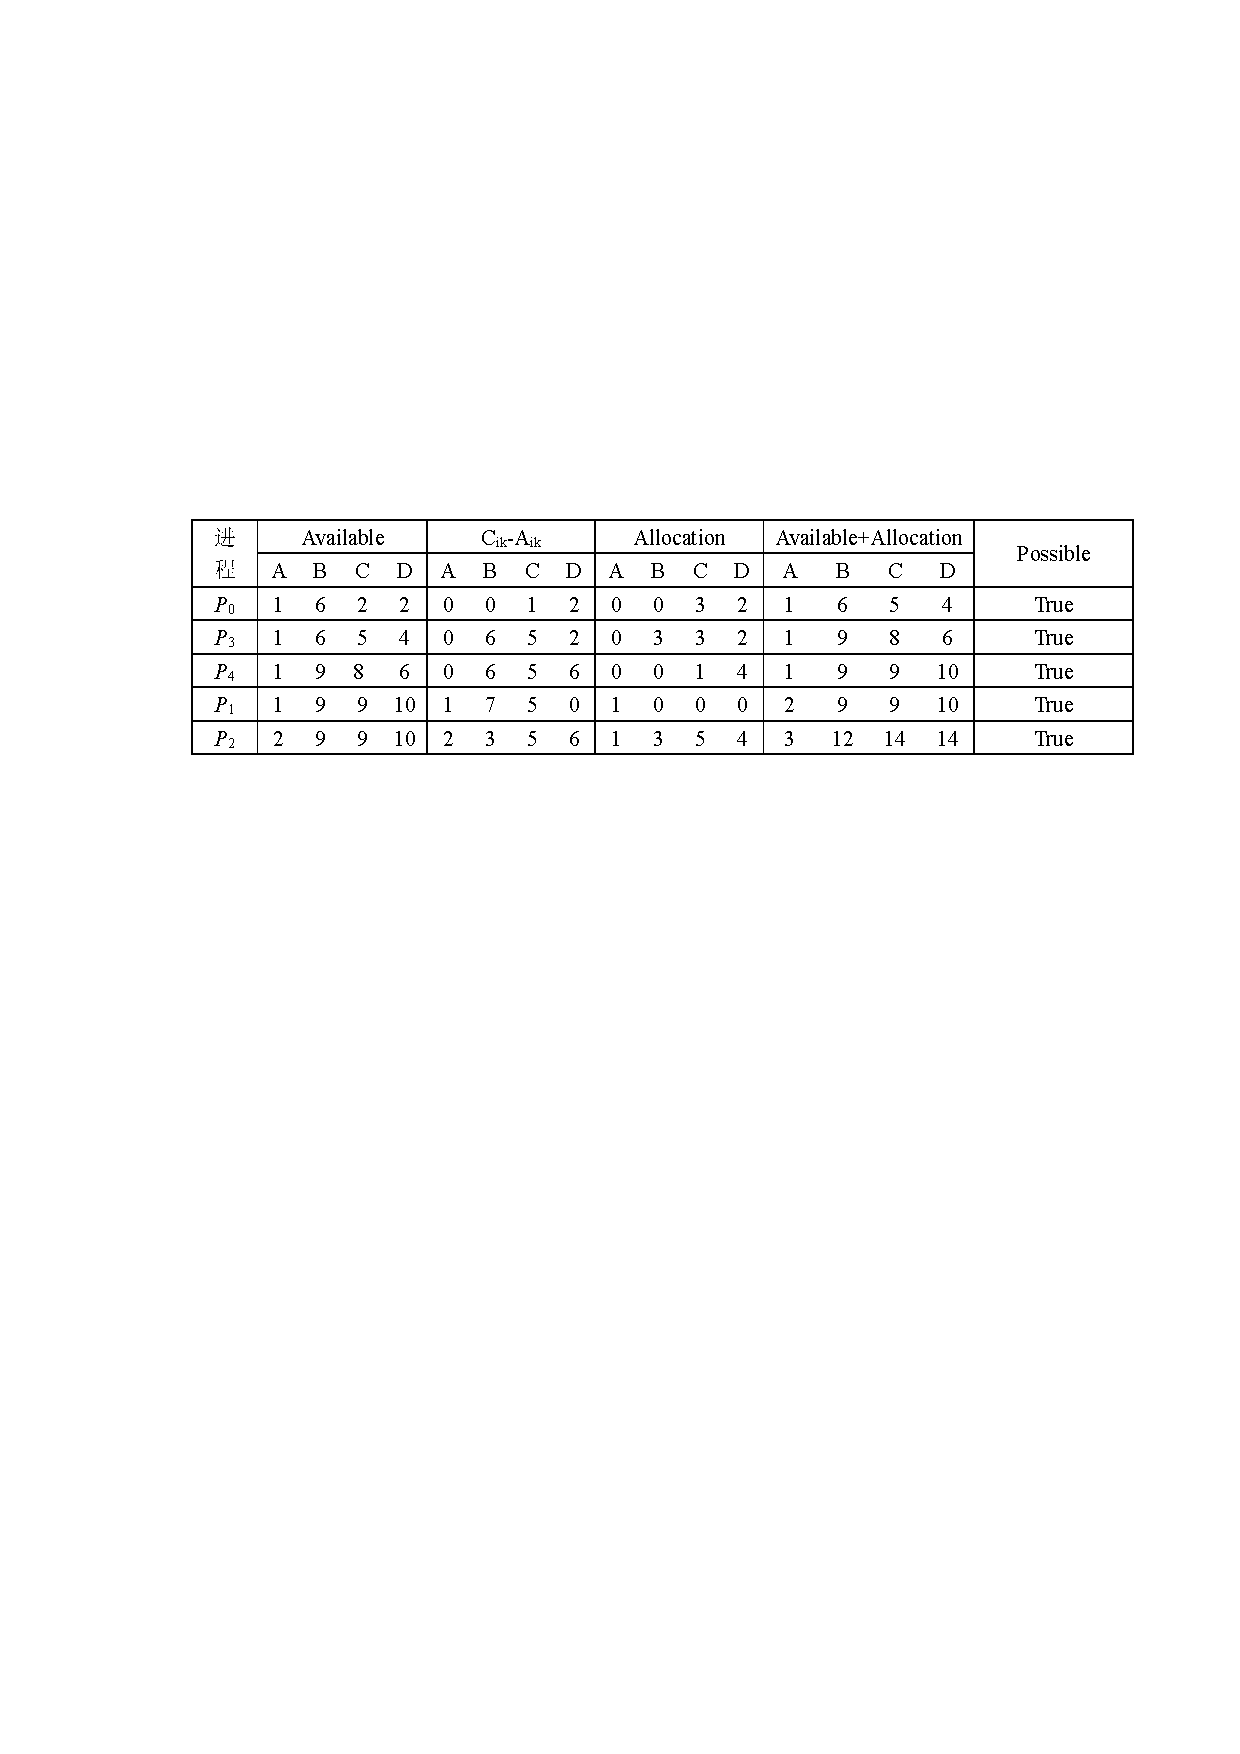
\includegraphics[width=0.95\linewidth]{img/10.2.pdf}
		\vspace{-1.5em}
	\end{figure}

	(2)不能分配。假设分配给进程$P_2$,此时$Available=(0, 4, 0, 0)$,不能满足任何一个进程,此时系统处于不安全状态,因此不能分配。
\end{solution}



\end{document}